\documentclass[notoc,notitlepage]{tufte-book}
% \nonstopmode % uncomment to enable nonstopmode

\usepackage{classnotetitle}

\title{PMATH467 --- Algebraic Geometry}
\author{Johnson Ng}
\subtitle{Classnotes for Winter 2019}
\credentials{BMath (Hons), Pure Mathematics major, Actuarial Science Minor}
\institution{University of Waterloo}

\setcounter{secnumdepth}{3}
\setcounter{tocdepth}{3}

\renewcommand{\baselinestretch}{1.1}
\usepackage{geometry}
\geometry{letterpaper}
\usepackage[parfill]{parskip}
\usepackage{graphicx}

% Essential Packages
\usepackage{makeidx}
\makeindex
\usepackage{enumitem}
\usepackage[T1]{fontenc}
\usepackage{natbib}
\bibliographystyle{apalike}
\usepackage{ragged2e}
\usepackage{etoolbox}
\usepackage{amssymb}
\usepackage{fontawesome}
\usepackage{amsmath}
\usepackage{mathrsfs}
\usepackage{mathtools}
\usepackage{xparse}
\usepackage{tkz-euclide}
\usetkzobj{all}
\usepackage[utf8]{inputenc}
\usepackage{csquotes}
\usepackage[english]{babel}
\usepackage{marvosym}
\usepackage{pgf,tikz}
\usepackage{pgfplots}
\usepackage{fancyhdr}
\usepackage{array}
\usepackage{faktor}
\usepackage{float}
\usepackage{xcolor}
\usepackage{centernot}
\usepackage{silence}
  \WarningFilter*{latex}{Marginpar on page \thepage\space moved}
\usepackage{tcolorbox}
\tcbuselibrary{skins,breakable}
\usepackage{longtable}
\usepackage[amsmath,hyperref]{ntheorem}
\usepackage{hyperref}
\usepackage[noabbrev,capitalize,nameinlink]{cleveref}

% xcolor (scheme: base16 eighties)
\definecolor{base16-eighties-dark}{HTML}{2D2D2D}
\definecolor{base16-eighties-light}{HTML}{D3D0C8}
\definecolor{base16-eighties-magenta}{HTML}{CD98CD}
\definecolor{base16-eighties-red}{HTML}{F47678}
\definecolor{base16-eighties-yellow}{HTML}{E2B552}
\definecolor{base16-eighties-green}{HTML}{98CD97}
\definecolor{base16-eighties-lightblue}{HTML}{61CCCD}
\definecolor{base16-eighties-blue}{HTML}{6498CE}
\definecolor{base16-eighties-brown}{HTML}{D47B4E}
\definecolor{base16-eighties-gray}{HTML}{747369}

% hyperref Package Settings
\hypersetup{
    bookmarks=true,         % show bookmarks bar?
    unicode=true,          % non-Latin characters in Acrobat’s bookmarks
    pdftoolbar=false,        % show Acrobat’s toolbar?
    pdfmenubar=false,        % show Acrobat’s menu?
    pdffitwindow=true,     % window fit to page when opened
    colorlinks=true,
    allcolors=base16-eighties-magenta,
}

% tikz
\usepgfplotslibrary{polar}
\usepgflibrary{shapes.geometric}
\usetikzlibrary{angles,patterns,calc,decorations.markings}
\tikzset{midarrow/.style 2 args={
        decoration={markings,
            mark= at position #2 with {\arrow{#1}} ,
        },
        postaction={decorate}
    },
    midarrow/.default={latex}{0.5}
}
\def\centerarc[#1](#2)(#3:#4:#5)% Syntax: [draw options] (center) (initial angle:final angle:radius)
    { \draw[#1] ($(#2)+({#5*cos(#3)},{#5*sin(#3)})$) arc (#3:#4:#5); }

% enumitems
\newlist{inlinelist}{enumerate*}{1}
\setlist*[inlinelist,1]{%
  label=(\roman*),
}

% Theorem Style Customization
\setlength\theorempreskipamount{2ex}
\setlength\theorempostskipamount{3ex}

\makeatletter
\let\nobreakitem\item
\let\@nobreakitem\@item
\patchcmd{\nobreakitem}{\@item}{\@nobreakitem}{}{}
\patchcmd{\nobreakitem}{\@item}{\@nobreakitem}{}{}
\patchcmd{\@nobreakitem}{\@itempenalty}{\@M}{}{}
\patchcmd{\@xthm}{\ignorespaces}{\nobreak\ignorespaces}{}{}
\patchcmd{\@ythm}{\ignorespaces}{\nobreak\ignorespaces}{}{}

\renewtheoremstyle{break}%
  {\item{\theorem@headerfont
          ##1\ ##2\theorem@separator}\hskip\labelsep\relax\nobreakitem}%
  {\item{\theorem@headerfont
          ##1\ ##2\ (##3)\theorem@separator}\hskip\labelsep\relax\nobreakitem}
\makeatother

% ntheorem + framed
\makeatletter

% ntheorem Declarations
\theorempreskip{10pt}
\theorempostskip{5pt}
\theoremstyle{break}

\newtheorem*{solution}{\faPencil $\enspace$ Solution}
\newtheorem*{remark}{Remark}
\newtheorem{eg}{Example}[section]
\newtheorem{ex}{Exercise}[section]

    % definition env
\theoremprework{\textcolor{base16-eighties-blue}{\hrule height 2pt}}
\theoremheaderfont{\color{base16-eighties-blue}\normalfont\bfseries}
\theorempostwork{\textcolor{base16-eighties-blue}{\hrule height 2pt}}
\theoremindent10pt
\newtheorem{defn}{\faBook \enspace Definition}

    % definition env no num
\theoremprework{\textcolor{base16-eighties-blue}{\hrule height 2pt}}
\theoremheaderfont{\color{base16-eighties-blue}\normalfont\bfseries}
\theorempostwork{\textcolor{base16-eighties-blue}{\hrule height 2pt}}
\theoremindent10pt
\newtheorem*{defnnonum}{\faBook \enspace Definition}

    % theorem envs
\theoremprework{\textcolor{base16-eighties-magenta}{\hrule height 2pt}}
\theoremheaderfont{\color{base16-eighties-magenta}\normalfont\bfseries}
\theorempostwork{\textcolor{base16-eighties-magenta}{\hrule height 2pt}}
\theoremindent10pt
\newtheorem{thm}{\faCoffee \enspace Theorem}

\theoremprework{\textcolor{base16-eighties-magenta}{\hrule height 2pt}}
\theorempostwork{\textcolor{base16-eighties-magenta}{\hrule height 2pt}}
\theoremindent10pt
\newtheorem{propo}[thm]{\faTint \enspace Proposition}

\theoremprework{\textcolor{base16-eighties-magenta}{\hrule height 2pt}}
\theorempostwork{\textcolor{base16-eighties-magenta}{\hrule height 2pt}}
\theoremindent10pt
\newtheorem{crly}[thm]{\faSpaceShuttle \enspace Corollary}

\theoremprework{\textcolor{base16-eighties-magenta}{\hrule height 2pt}}
\theorempostwork{\textcolor{base16-eighties-magenta}{\hrule height 2pt}}
\theoremindent10pt
\newtheorem{lemma}[thm]{\faTree \enspace Lemma}

\theoremprework{\textcolor{base16-eighties-magenta}{\hrule height 2pt}}
\theorempostwork{\textcolor{base16-eighties-magenta}{\hrule height 2pt}}
\theoremindent10pt
\newtheorem{axiom}[thm]{\faShield \enspace Axiom}

    % theorem envs without counter
\theoremprework{\textcolor{base16-eighties-magenta}{\hrule height 2pt}}
\theoremheaderfont{\color{base16-eighties-magenta}\normalfont\bfseries}
\theorempostwork{\textcolor{base16-eighties-magenta}{\hrule height 2pt}}
\theoremindent10pt
\newtheorem*{thmnonum}{\faCoffee \enspace Theorem}

\theoremprework{\textcolor{base16-eighties-magenta}{\hrule height 2pt}}
\theorempostwork{\textcolor{base16-eighties-magenta}{\hrule height 2pt}}
\theoremindent10pt
\newtheorem*{propononum}{\faTint \enspace Proposition}

\theoremprework{\textcolor{base16-eighties-magenta}{\hrule height 2pt}}
\theorempostwork{\textcolor{base16-eighties-magenta}{\hrule height 2pt}}
\theoremindent10pt
\newtheorem*{crlynonum}{\faSpaceShuttle \enspace Corollary}

\theoremprework{\textcolor{base16-eighties-magenta}{\hrule height 2pt}}
\theorempostwork{\textcolor{base16-eighties-magenta}{\hrule height 2pt}}
\theoremindent10pt
\newtheorem*{lemmanonum}{\faTree \enspace Lemma}

\theoremprework{\textcolor{base16-eighties-magenta}{\hrule height 2pt}}
\theorempostwork{\textcolor{base16-eighties-magenta}{\hrule height 2pt}}
\theoremindent10pt
\newtheorem*{axiomnonum}{\faShield \enspace Axiom}

    % proof env
\theoremprework{\textcolor{base16-eighties-brown}{\hrule height 2pt}}
\theoremheaderfont{\color{base16-eighties-brown}\normalfont\bfseries}
\theorempostwork{\textcolor{base16-eighties-brown}{\hrule height 2pt}}
\newtheorem*{proof}{\faPencil \enspace Proof}

    % note and notation env
\theoremprework{\textcolor{base16-eighties-yellow}{\hrule height 2pt}}
\theoremheaderfont{\color{base16-eighties-yellow}\normalfont\bfseries}
\theorempostwork{\textcolor{base16-eighties-yellow}{\hrule height 2pt}}
\newtheorem*{note}{\faQuoteLeft \enspace Note}

\theoremprework{\textcolor{base16-eighties-yellow}{\hrule height 2pt}}
\theorempostwork{\textcolor{base16-eighties-yellow}{\hrule height 2pt}}
\newtheorem*{notation}{\faPaw \enspace Notation}

    % warning env
\theoremprework{\textcolor{base16-eighties-red}{\hrule height 2pt}}
\theoremheaderfont{\color{base16-eighties-red}\normalfont\bfseries}
\theorempostwork{\textcolor{base16-eighties-red}{\hrule height 2pt}}
\theoremindent10pt
\newtheorem*{warning}{\faBug \enspace Warning}

% more environments
\newtcolorbox{redquote}{
  blanker,enhanced,breakable,standard jigsaw,
  opacityback=0,
  coltext=base16-eighties-light,
  left=5mm,right=5mm,top=2mm,bottom=2mm,
  colframe=base16-eighties-red,
  boxrule=0pt,leftrule=3pt,
  fontupper=\itshape
}
\newtcolorbox{bluequote}{
  blanker,enhanced,breakable,standard jigsaw,
  opacityback=0,
  coltext=base16-eighties-light,
  left=5mm,right=5mm,top=2mm,bottom=2mm,
  colframe=base16-eighties-blue,
  boxrule=0pt,leftrule=3pt,
  fontupper=\itshape
}
\newtcolorbox{greenquote}{
  blanker,enhanced,breakable,standard jigsaw,
  opacityback=0,
  coltext=base16-eighties-light,
  left=5mm,right=5mm,top=2mm,bottom=2mm,
  colframe=base16-eighties-green,
  boxrule=0pt,leftrule=3pt,
  fontupper=\itshape
}
\newtcolorbox{yellowquote}{
  blanker,enhanced,breakable,standard jigsaw,
  opacityback=0,
  coltext=base16-eighties-light,
  left=5mm,right=5mm,top=2mm,bottom=2mm,
  colframe=base16-eighties-yellow,
  boxrule=0pt,leftrule=3pt,
  fontupper=\itshape
}
\newtcolorbox{magentaquote}{
  blanker,enhanced,breakable,standard jigsaw,
  opacityback=0,
  coltext=base16-eighties-light,
  left=5mm,right=5mm,top=2mm,bottom=2mm,
  colframe=base16-eighties-magenta,
  boxrule=0pt,leftrule=3pt,
  fontupper=\itshape
}

% ntheorem listtheorem style
\makeatother
\newlength\widesttheorem
\AtBeginDocument{
  \settowidth{\widesttheorem}{Proposition A.1.1.1\quad}
}

\makeatletter
\def\thm@@thmline@name#1#2#3#4{%
        \@dottedtocline{-2}{0em}{2.3em}%
                   {\makebox[\widesttheorem][l]{#1 \protect\numberline{#2}}#3}%
                   {#4}}
\@ifpackageloaded{hyperref}{
\def\thm@@thmline@name#1#2#3#4#5{%
    \ifx\#5\%
        \@dottedtocline{-2}{0em}{2.3em}%
            {\makebox[\widesttheorem][l]{#1 \protect\numberline{#2}}#3}%
            {#4}
    \else
        \ifHy@linktocpage\relax\relax
            \@dottedtocline{-2}{0em}{2.3em}%
                {\makebox[\widesttheorem][l]{#1 \protect\numberline{#2}}#3}%
                {\hyper@linkstart{link}{#5}{#4}\hyper@linkend}%
        \else
            \@dottedtocline{-2}{0em}{2.3em}%
                {\hyper@linkstart{link}{#5}%
                  {\makebox[\widesttheorem][l]{#1 \protect\numberline{#2}}#3}\hyper@linkend}%
                    {#4}%
        \fi
    \fi}
}

\makeatletter
\def\thm@@thmline@noname#1#2#3#4{%
        \@dottedtocline{-2}{0em}{5em}%
                   {{\protect\numberline{#2}}#3}%
                   {#4}}
\@ifpackageloaded{hyperref}{
\def\thm@@thmline@noname#1#2#3#4#5{%
    \ifx\#5\%
        \@dottedtocline{-2}{0em}{5em}%
            {{\protect\numberline{#2}}#3}%
            {#4}
    \else
        \ifHy@linktocpage\relax\relax
            \@dottedtocline{-2}{0em}{5em}%
                {{\protect\numberline{#2}}#3}%
                {\hyper@linkstart{link}{#5}{#4}\hyper@linkend}%
        \else
            \@dottedtocline{-2}{0em}{5em}%
                {\hyper@linkstart{link}{#5}%
                  {{\protect\numberline{#2}}#3}\hyper@linkend}%
                    {#4}%
        \fi
    \fi}
}

\theoremlisttype{allname}

\AtBeginDocument{\renewcommand\contentsname{Table of Contents}}

% Heading formattings
% chapter format
\titleformat{\chapter}%
  {\huge\rmfamily\itshape\color{base16-eighties-magenta}}% format applied to label+text
  {\llap{\colorbox{base16-eighties-magenta}{\parbox{1.5cm}{\hfill\itshape\huge\textcolor{base16-eighties-dark}{\thechapter}}}}}% label
  {5pt}% horizontal separation between label and title body
  {}% before the title body
  []% after the title body

% section format
\titleformat{\section}%
  {\normalfont\Large\rmfamily\itshape\color{base16-eighties-blue}}% format applied to label+text
  {\llap{\colorbox{base16-eighties-blue}{\parbox{1.5cm}{\hfill\itshape\textcolor{base16-eighties-dark}{\thesection}}}}}% label
  {5pt}% horizontal separation between label and title body
  {}% before the title body
  []% after the title body

% subsection format
\titleformat{\subsection}%
  {\normalfont\large\itshape\color{base16-eighties-green}}% format applied to label+text
  {\llap{\colorbox{base16-eighties-green}{\parbox{1.5cm}{\hfill\textcolor{base16-eighties-dark}{\thesubsection}}}}}% label
  {1em}% horizontal separation between label and title body
  {}% before the title body
  []% after the title body

% Sidenote enhancements
\def\mathmarginnote#1{%
  \tag*{\rlap{\hspace\marginparsep\smash{\parbox[t]{\marginparwidth}{%
  \footnotesize#1}}}}
}

% Custom table columning
\newcolumntype{L}[1]{>{\raggedright\let\newline\\\arraybackslash\hspace{0pt}}m{#1}}
\newcolumntype{C}[1]{>{\centering\let\newline\\\arraybackslash\hspace{0pt}}m{#1}}
\newcolumntype{R}[1]{>{\raggedleft\let\newline\\\arraybackslash\hspace{0pt}}m{#1}}

% Custom math operator
% \DeclareMathOperator{\rem}{rem}
\DeclareMathOperator*{\argmax}{arg\,max}
\DeclareMathOperator*{\argmin}{arg\,min}
\DeclareMathOperator{\re}{Re}
\DeclareMathOperator{\im}{Im}
\DeclareMathOperator{\caparg}{Arg}
\DeclareMathOperator{\Ind}{Ind}
\DeclareMathOperator{\Res}{Res}

% Graph styles
\pgfplotsset{compat=1.15}
\usepgfplotslibrary{fillbetween}
\pgfplotsset{four quads/.append style={axis x line=middle, axis y line=
middle, xlabel={$x$}, ylabel={$y$}, axis equal }}
\pgfplotsset{four quad complex/.append style={axis x line=middle, axis y line=
middle, xlabel={$\re$}, ylabel={$\im$}, axis equal }}

% Shortcuts
\newcommand{\floor}[1]{\lfloor #1 \rfloor}      % simplifying the writing of a floor function
\newcommand{\ceiling}[1]{\lceil #1 \rceil}      % simplifying the writing of a ceiling function
\newcommand{\dotp}{\, \cdotp}			        % dot product to distinguish from \cdot
\newcommand{\qed}{\hfill\ensuremath{\square}}   % Q.E.D sign
\newcommand{\abs}[1]{\left|#1\right|}						% absolute value
\newcommand{\lra}[1]{\langle \; #1 \; \rangle}
\newcommand{\at}[2]{\Big|_{#1}^{#2}}
\newcommand{\Arg}[1]{\caparg #1}
\renewcommand{\bar}[1]{\mkern 1.5mu \overline{\mkern -1.5mu #1 \mkern -1.5mu} \mkern 1.5mu}
\newcommand{\quotient}[2]{\faktor{#1}{#2}}
\newcommand{\cyclic}[1]{\left\langle #1 \right\rangle}
	% highlighting shortcuts
\newcommand{\hlimpo}[1]{\textcolor{base16-eighties-red}{\textbf{#1}}}
\newcommand{\hlwarn}[1]{\textcolor{base16-eighties-yellow}{\textbf{#1}}}
\newcommand{\hldefn}[1]{\textcolor{base16-eighties-blue}{\index{#1}\textbf{#1}}}
\newcommand{\hlnotea}[1]{\textcolor{base16-eighties-green}{\textbf{#1}}}
\newcommand{\hlnoteb}[1]{\textcolor{base16-eighties-lightblue}{\textbf{#1}}}
\newcommand{\hlnotec}[1]{\textcolor{base16-eighties-brown}{\textbf{#1}}}
\newcommand{\WTP}{\textcolor{base16-eighties-brown}{WTP} }
\newcommand{\WTS}{\textcolor{base16-eighties-brown}{WTS} }
\newcommand{\ind}[2]{\Ind_{#2}\left( #1 \right)}
\newcommand{\notimply}{\centernot\implies}
\newcommand{\res}[2]{\underset{#2}{\Res} #1 }
\newcommand{\tworow}[3]{\begin{tabular}{@{}#1@{}} #2 \\ #3 \end{tabular}}
\renewcommand{\epsilon}{\varepsilon}
\newcommand{\lrarrow}{\leftrightarrow}
\newcommand{\larrow}{\leftarrow}
\newcommand{\rarrow}{\rightarrow}
\renewcommand{\atop}[2]{\genfrac{}{}{0pt}{}{#1}{#2}}
\newcommand*\dif{\mathop{}\!d}

  % inspiration from: https://tex.stackexchange.com/questions/8720/overbrace-underbrace-but-with-an-arrow-instead#37758
\newcommand{\overarrow}[2]{
  \overset{\makebox[0pt]{\begin{tabular}{@{}c@{}}#2\\[0pt]\ensuremath{\uparrow}\end{tabular}}}{#1}
}
\newcommand{\underarrow}[2]{
  \underset{\makebox[0pt]{\begin{tabular}{@{}c@{}}\downarrow\\[0pt]\ensuremath{#2}\end{tabular}}}{#1}
}

% Document header formatting
\renewcommand{\chaptermark}[1]{\markboth{#1}{}}
\renewcommand{\sectionmark}[1]{\markright{#1}}
\makeatletter
\pagestyle{fancy}
\fancyhead{}
\fancyhead[RO]{\textsl{\@title} \enspace \thepage}
\fancyhead[LE]{\thepage \enspace \textsl{\leftmark \enspace - \enspace \rightmark}}
\makeatother

% Comment the two lines below if you want to print the document
\pagecolor{base16-eighties-dark}
\color{base16-eighties-light}


\DeclareMathOperator{\id}{id}

\DeclareMathOperator{\Int}{Int}

\begin{document}
\hypersetup{pageanchor=false}
\maketitle
\hypersetup{pageanchor=true}
\begin{fullwidth}
\tableofcontents
\end{fullwidth}

\newpage
\begin{fullwidth}
  \renewcommand{\listtheoremname}{\faBook\ \slshape List of Definitions}
  \listoftheorems[ignoreall,show={defn}]
  \addcontentsline{toc}{chapter}{List of Definitions}
\end{fullwidth}

\newpage 
\begin{fullwidth}
  \renewcommand{\listtheoremname}{\faCoffee\ \slshape List of Theorems}
  \listoftheorems[ignoreall,
    show={axiom,lemma,thm,crly,propo,marginthm,marginpropo,marginlemma,marginaxiom,margincrly}
  ]
  \addcontentsline{toc}{chapter}{List of Theorems}
\end{fullwidth}


\chapter*{Preface}%
\addcontentsline{toc}{chapter}{Preface}
\label{chp:preface}
% chapter preface

The basic goal of the course is to be able to find \hlnotea{algebraic invariants}, which we shall use to classify topological spaces up to homeomorphism.

Other questions that we shall also look into include a uniqueness problem about manifolds; in particular, how many manifolds exist for a given invariant up to homeomorphism? We shall see that for a \hlnotea{2-manifold}, the only such manifold is the 2-dimensional sphere $S^2$. For a $4$-manifold, it is the $4$-dimensional sphere $S^4$. In fact, for any other $n$-manifold for $n > 4$, the unique manifold is the respective $n$-sphere. The problem is trickier with the $3$-manifold, and it is known as the Poincar\'{e} Conjecture, solved in 2003 by Russian Mathematician \href{https://en.wikipedia.org/wiki/Grigori_Perelman}{Grigori Perelman}. Indeed, the said manifold is homeomorphic to the $3$-sphere.

For this course, you are expected to be familiar with notions from \hlnotea{real analysis},
such as topology, and concepts from \hlnotea{group theory}. Due to the structure of which this
course is designed, each lecture may be much longer than reality, as I am also making heavy
references to the recommended text that is Lee's Introduction to Topological Manifolds
\cite{johnlee2000}.

The following topics shall be covered:
\begin{enumerate}
  \item Point-Set Topology
  \item Introduction to Topological Manifolds
  \item Simplicial complexes \& Introduction to Homology
  \item Fundamental Groups \& Covering Spaces
  \item Classification of Surfaces
\end{enumerate}

\textbf{\newthought{Feb 12th}} I have decided to delve deeper into the recommended text
as the organization of the course demands. As so, changes might be made to earlier
lectures as I go further down, so as to introduce the definitions and provide propositions
at a timing deemed appropriate. To keep track of the changes, please look for
\hlnotea{PMATH467} among the commits on
\url{https://gitlab.com/japorized/TeX_notes/commits/master} using the provided filter. If
you are unfamiliar with version controlling and writing in \LaTeX, once you have found the
lecture that you wish to compare, expand the \hlnotea{diff} for \texttt{classnotes.tex}
if it is collapsed.

\section*{Basic Logistics for the Course}%
% section basic_logistics_for_the_course

I shall leave this here for my own notes, in case something happens to my hard copy.

\begin{itemize}
  \item OH: (Tue) 1630 - 1800, (Fri) 1245 - 1320
  \item OR: MC 6457
  \item EM: aaleyasin
\end{itemize}

% section basic_logistics_for_the_course (end)

% chapter preface (end)

\tuftepart{Point-Set Topology}

\chapter{Lecture 1 Jan 07th}%
\label{chp:lecture_1_jan_07th}
% chapter lecture_1_jan_07th
\nocite{johnlee2000}

We will not be too rigorous in this part.

\section{Euclidean Space}%
\label{sec:euclidean_space}
% section euclidean_space

For any $(x_1, \ldots, x_m) \in \mathbb{R}^m$, we can measure its distance from the origin $0$ using either
\begin{itemize}
  \item $\norm{x}_\infty = \max \{ \abs{ x_i } \}$ (the supremum-norm);
  \item $\norm{x}_2 = \sqrt{ \sum (x_j)^2 }$ (the $2$-norm); or
  \item $\norm{x}_p = \left( \sum \abs{ x_j }^p \right)^\frac{1}{p}$ (the $p$-norm),
\end{itemize}
where we may define a ``distance'' by
\begin{equation*}
  d_p(x, y) = \norm{ x - y }_p.
\end{equation*}

\begin{defn}[Metric]\index{Metric}\label{defn:metric}
  Let $X$ be an arbitrary space. A function $d : X \times X \to \mathbb{R}$ is called a \hlnoteb{metric} if it satisfies
  \begin{enumerate}
    \item (symmetry) $d(x, y) = d(y, x)$ for any $x, y \in X$;
    \item (positive definiteness) $d(x, y) \geq 0$ for any $x, y \in X$, and $d(x, y) = 0 \iff x = y$; and
    \item (triangle inequality) $\forall x, y, z \in X$
      \begin{equation*}
        d(x, y) \leq d(x, z) + d(y, z).
      \end{equation*}
  \end{enumerate}
\end{defn}

\begin{defn}[Open and Closed Sets]\index{Open sets}\index{Closed sets}\label{defn:open_and_closed_sets}
  Given a space $X$ with a metric $d$, and $r > 0$, the set
  \begin{equation*}
    B(x, r) := \{ w \in X \mid d(x, w) < r \}
  \end{equation*}
  is called the \hlnoteb{open ball} of radius $r$ centered at $x$. An \hlnoteb{open set} $A$ is such that $\forall a \in A$, $\exists r > 0$ such that
  \begin{equation*}
    B(a, r) \subseteq A.
  \end{equation*}
  We say that a set is \hlnoteb{closed} if its complement is open.
\end{defn}

\begin{defn}[Continuous Map]\index{Continuous Map}\label{defn:continuous_map}
  A function
  \begin{equation*}
    f : (X, d_1) \to (Y, d_2)
  \end{equation*}
  is said to be \hlnoteb{continuous} if the preimage of an open set in $Y$ is open in $X$.\marginnote{See \href{https://tex.japorized.ink/PMATH351F18/classnotes.pdf\#thm.45}{notes} on Real Analysis for why we defined a continuous map in such a way.}
\end{defn}

\begin{warning}
  This definition does not imply that a continuous map $f$ maps open sets to open sets.
\end{warning}

\begin{defn}[Open and Closed Maps]\index{Open Map}\index{Closed Maps}\label{defn:open_and_closed_maps}
  A mapping $f : X \to Y$ is said to be \hlnoteb{open} if for all open $U \subset X$, $f(U)$ is
  open. We say that $f$ is a \hlnoteb{closed map} if for all closed $F \subset X$, $f(F)$ is
  closed.
\end{defn}
\marginnote{
\begin{ex}\label{ex:homeomorphm_iff_open_and_closed}
  Suppose $f : X \to Y$ is a bijective continuous map. Then TFAE.
  \begin{enumerate}
    \item $f$ is a homeomorphism.
    \item $f$ is open.
    \item $f$ is closed.
  \end{enumerate}
\end{ex}
}

\begin{ex}
  Contruct a function on $[0, 1]$ which assumes all values between its maximum and minimum, but is not continuous.
\end{ex}

\begin{solution}
  Consider the piecewise function
  \begin{equation*}
    f(x) = \begin{cases}
      x & 0 \leq x < \frac{1}{2} \\
      x - \frac{1}{2} & x \geq \frac{1}{2}.
    \end{cases}
  \end{equation*}
  It is clear that the maximum and minimum are $\frac{1}{2}$ and $0$ respectively, and $f$ assumes all values between $0$ and $\frac{1}{2}$. However, a piecewise function is not continuous.
\end{solution}

\begin{defn}[Homeomorphism]\index{Homeomorphism}\label{defn:homeomorphism}
  A function $f$ is a \hlnoteb{homeomorphism} if it is a bijection and both $f$ and $f^{-1}$ are continuous.
\end{defn}

\begin{eg}
  The function
  \begin{equation*}
    g : [ 0, 2\pi ) \to \mathbb{R}^2 \text{ given by } \theta \mapsto (\cos \theta, \sin \theta)
  \end{equation*}
  is not homeomorphic, since if we consider an alternating series that converges to $0$ on the unit circle on $\mathbb{R}^2$, we have that the preimage of the series does not converge and $f^{-1}$ is in fact discontinuous.
\end{eg}

% TODO: define convergence; see Introduction to Topological Manifolds by J. Lee pg. 20

\newthought{Now}, we want to talk about topologies without referring to a metric.

\begin{defn}[Topology]\index{Topology}\label{defn:topology}
  Let $X$ be a space. We say that the set $\mathcal{T} \subseteq \mathcal{P}(X)$ is a \hlnoteb{topology} if
  \begin{enumerate}
    \item $X, \emptyset \in \mathcal{T}$;
    \item if $\left\{ x_\alpha \right\}_{\alpha \in A} \subseteq \mathcal{T}$ for an arbitrary index set $A$, then
      \begin{equation*}
        \bigcup_{\alpha \in A} x_\alpha \in \mathcal{T}; \text{ and }
      \end{equation*}
    \item If $\{ x_\beta \}_{\beta \in B} \subset \mathcal{T}$ for some finite index set $B$, then
      \begin{equation*}
        \bigcap_{\beta \in B} x_\beta \in \mathcal{T}.
      \end{equation*}
  \end{enumerate}
\end{defn}

% section euclidean_space (end)

% chapter lecture_1_jan_07th (end)

\chapter{Lecture 2 Jan 09th}%
\label{chp:lecture_2_jan_09th}
% chapter lecture_2_jan_09th

\section{Euclidean Space (Continued)}%
\label{sec:euclidean_space_continued}
% section euclidean_space_continued

In the last lecture, from metric topology, we generalized the notion to a more abstract one
that is based solely on open sets.

\begin{eg}
  Let $X$ be a set. The following two are
  uninteresting examples of topologies:
  \begin{enumerate}
    \item The \hldefn{trivial topology} $\mathcal{T} = \left\{ \emptyset, X \right\}$.
    \item The \hldefn{discrete topology} $\mathcal{T} = \mathcal{P}(X)$.
  \end{enumerate}
\end{eg}

\newthought{We shall now} continue with looking at
more concepts that we shall need down the road.

\begin{defn}[Closure of a Set]\index{Closure}\label{defn:closure_of_a_set}
  Let $A$ be a set. Its \hlnoteb{closure},
  denoted as $\bar{A}$, is defined as
  \begin{equation*}
    \bar{A} = \bigcap_{C \supset A}^{C: \text{ closed }} C.
  \end{equation*}
  It is the smallest closed set that contains $A$.
\end{defn}

\begin{note}
  In metric topology, one typically defines the closure of a set by taking the union of $A$ and its limit points.
\end{note}

\begin{defn}[Interior of a Set]\index{Interior}\label{defn:interior_of_a_set}
  Let $A$ be a set. Its \hlnoteb{interior},
  denoted either as $\text{Int }(A)$, $A^\circ$ or $\Int(A)$,
  is defined as
  \begin{equation*}
    \Int(A) = \bigcup_{G \subseteq A}^{G: \text{ open }} G.
  \end{equation*}
\end{defn}

\begin{defn}[Boundary of a Set]\index{Boundary}\label{defn:boundary_of_a_set}
  Let $A$ be a set. Its \hlnoteb{boundary},
  denoted as $\partial A$, is defined as
  \begin{equation*}
    \partial A = \bar{A} \setminus \Int(A).
  \end{equation*}
\end{defn}

\begin{ex}
  Let $A$ be a set. Prove that $\partial A$ is closed.
\end{ex}

\begin{proof}
  Notice that
  \begin{equation*}
    ( \partial A )^C = ( \bar{A} \setminus \Int(A) )^C = X \setminus \bar{A} \cup \Int(A) = X \cap \bar{A}^C \cup \Int(A)
  \end{equation*}
  which is open.
\end{proof}

\begin{ex}
  Let $A$ be a set. Show that
  \begin{equation*}
    \partial ( \partial A ) = \partial A.
  \end{equation*}
\end{ex}

\begin{proof}
  First, notice that $\Int(\partial A) = \emptyset$.
  Since $\partial A$ is closed, $\bar{\partial A} = \partial A$.
  Then
  \begin{equation*}
    \partial ( \partial A ) = \bar{\partial A} \setminus \Int(\partial A)
      = \partial A \setminus \emptyset = \partial A
  \end{equation*}
\end{proof}

\begin{eg}
  We know that $\mathbb{Q} \subseteq \mathbb{R}$,
  and $\bar{\mathbb{Q}} = \mathbb{R}$.
  We say that $\mathbb{Q}$ is dense in $\mathbb{R}$.
\end{eg}

\begin{defn}[Dense]\index{Dense}\label{defn:dense}
  We say that a subset $A$ of a set $X$ is dense if
  \begin{equation*}
    \bar{A} = X.
  \end{equation*}
\end{defn}

\begin{eg}
  From the last example, we have that $\Int(\mathbb{Q}) = \emptyset$.
\end{eg}

\begin{defn}[Limit Point]\index{Limit Point}\label{defn:limit_point}
  We say that $p \in X \supseteq A$ is a limit point of $A$
  if any neighbourhood of $p$ has a nontrivial intersection
  with $A$.
\end{defn}

\begin{eg}[A Topologist's Circle]\label{eg:a_topologists_circle}
  Consider the function
  \begin{equation*}
    f(x) = \begin{cases}
      \sin \frac{1}{x} & x \neq 0 \\
      0                & x = 0
    \end{cases}
  \end{equation*}
  on the interval $\left[ -\frac{1}{2 \pi}, \frac{1}{2 \pi} \right]$.
  Extend the function on both ends such that we obtain \cref{fig:a_topologists_circle}
  (See also: \href{https://www.desmos.com/calculator/figksl5wmv}{Desmos}).
  \begin{figure}[ht]
    \centering
    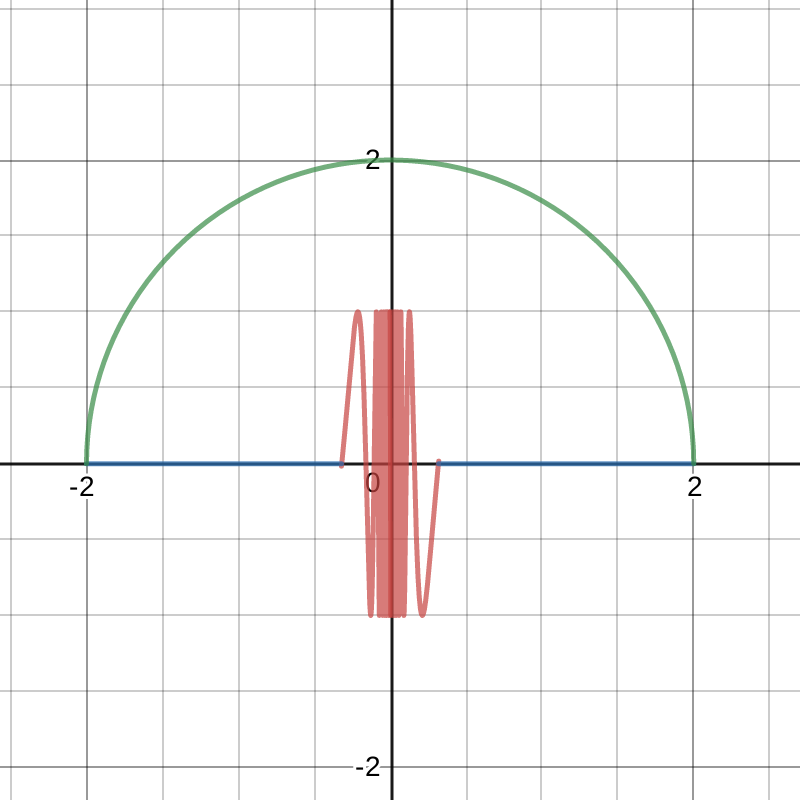
\includegraphics[width=0.7\linewidth]{topologists-circle.png}
    \caption{A Topologist's Circle}
    \label{fig:a_topologists_circle}
  \end{figure}

  The limit points of the graph includes all the points
  on the straight line from $(0, -1)$ to $(0, 1)$, including the endpoints.
  This is the case because for any of the points on this line, for any
  neighbourhood around the point, the neighbourhood intersects the
  graph $f$ infinitely many times.
\end{eg}

\newthought{Going back to continuity}, given a function $f$,
how do we know if $f^{-1}$ maps an open set to an open set?

We can actually reduce the problem to only looking at open balls.
But why are we allowed to do that?

\begin{defn}[Basis of a Topology]\index{Basis}\label{defn:basis_of_a_topology}
  \marginnote{Note that while the definition is similar to that of a cover, we are now ``covering'' over sets and not points.}
  Given a topology $\mathcal{T}$, we say that
  $\mathcal{B} = \left\{ B_{\alpha} \right\}_{\alpha \in I}$
  is a \hlnoteb{basis} if $\forall T \in \mathcal{T}$, there
  exists $J \subset I$ such that
  \begin{equation*}
    T = \bigcup_{\alpha \in J} B_\alpha.
  \end{equation*}
\end{defn}

\begin{eg}\label{eg:basis_of_r_n}
  Let $\mathcal{T}$ be the Euclidean topology on $\mathbb{R}$.
  Then we can take
  \begin{equation*}
    \mathcal{B} = \left\{ (a, b) \mmid a, b \in \mathbb{R}, \, a \leq b \right\}.
  \end{equation*}
  Note that $\mathcal{B}$ is \hlnotea{uncountable}.
  We can, in fact, have
  \sidenote{Recall from
  \href{https://tex.japorized.ink/PMATH351F18/classnotes.pdf}{PMATH 351}
  that we can write $\mathbb{R}$ as a disjoint union
  of open intervals with rational endpoints.}
  \begin{equation*}
    \mathcal{B}_1 = \left\{ (a, b) \mmid a, b \in \mathbb{Q}, a \leq b \right\},
  \end{equation*}
  which is countable, as a basis for $\mathbb{R}$.
  Furthermore, we can consider the set
  \begin{equation*}
    \mathcal{B}_2 = \left\{ (a, b) \mmid a \leq b, \, a = \frac{m}{2^p}, \, b = \frac{n}{2^q}, \, m, n, p, q \in \mathbb{Z} \right\},
  \end{equation*}
  which is also a countable basis for $\mathbb{R}$.
  Notice that
  \begin{equation*}
    \mathcal{B}_2 \subseteq \mathcal{B}_1 \subseteq \mathcal{B}.
  \end{equation*}
\end{eg}

\begin{eg}
  In $\mathbb{R}^2$, we can do a similar construction of $\mathcal{B}$,
  $\mathcal{B}_1$, and $\mathcal{B}_2$ as in the last example and use
  them as a basis for $\mathbb{R}^2$. In particular, we would have
  \begin{equation*}
    \mathcal{B} = \left\{ (a_1, b_1) \times (a_2, b_2) \mmid a_1, a_2, b_1, b_2 \in \mathbb{R} \right\}.
  \end{equation*}
  This is called a \hldefn{dyadic partitioning} of $\mathbb{R}^2$.
\end{eg}

\begin{eg}
  Let $(X_1, \mathcal{T}_1)$ and $(X_2, \mathcal{T}_2)$ be two topological spaces.
  Then the Cartesian product $X_1 \times X_2$ has topology induced
  from $\mathcal{T}_1$ and $\mathcal{T}_2$ by taking the set
  \begin{equation*}
    \mathcal{B} = \left\{ \beta_1 \times \beta_2 \mmid \beta_1 \in \mathcal{T}_1, \, \beta_2 \in \mathcal{T}_2 \right\}
  \end{equation*}
  as the basis.
\end{eg}

\begin{ex}
  Prove that
  \begin{enumerate}
    \item $\beta_1$ and $\beta_2$ can be taken to be elements of
      bases $\mathcal{B}_1 \subset \mathcal{T}_1$ and
      $\mathcal{B}_2 \subset \mathcal{T}_2$, respectively.
    \item the product topology on $\mathbb{R}^2$ is the same
      as the Euclidean topology.
  \end{enumerate}
\end{ex}

% section euclidean_space_continued (end)

% chapter lecture_2_jan_09th (end)

\chapter{Lecture 3 Jan 11th}%
\label{chp:lecture_3_jan_11th}
% chapter lecture_3_jan_11th

\section{Euclidean Space (Continued 2)}%
\label{sec:euclidean_space_continued_2}
% section euclidean_space_continued_2

\marginnote{The student is recommended to do a quick review for the first 3
chapters of the recommended text.}

Let $\tilde{X}$ be a metric space, and $p, q \in \tilde{X}$ with $p \neq q$.
Then we have that $d(p, q) = r > 0$.
\begin{marginfigure}
  \centering
  \begin{tikzpicture}
    \node[circle,fill,inner sep=1pt,label={270:{$p$}}] at (0, 0) {};
    \node[circle,fill,inner sep=1pt,label={270:{$q$}}] at (2, 1) {};
    \draw[latex'-latex'] (0, 0) -- (2, 1) node[midway,fill=dark] {r};
    \draw[dashed] (0, 0) circle(0.7);
    \draw[dashed] (2, 1) circle(0.7);
  \end{tikzpicture}
  \caption{Idea of separation}\label{fig:idea_of_separation}
\end{marginfigure}
Then we must have that
\begin{equation*}
  B \left( p, \frac{r}{3} \right) \cap B \left( q, \frac{r}{3} \right) = \emptyset.
\end{equation*}

\begin{ex}
  Prove that the above claim is true. (Use the triangle inequality)
\end{ex}

\begin{proof}
  Suppose $\exists x \in B \left( p, \frac{r}{3} \right) \cap B \left( q, \frac{r}{3} \right)$.
  Then
  \begin{equation*}
    d(p, x) + d(q, x) < \frac{2r}{3} < r = d(p, q),
  \end{equation*}
  which violates the triangle inequality.
\end{proof}

We observe here that the two open sets (or balls) ``separate'' $p$ and $q$.

\begin{defn}[Hausdorff / $T_2$]\index{Hausdorff}\index{$T_2$}\label{defn:hausdorff_t_2_}
  Let $X$ be a topological space. $X$ is said to be \hlnoteb{Hausdorff} or \hlnoteb{$T_2$}
  iff any $2$ distinct points can be separated by disjoint open sets.
\end{defn}

\begin{note}
  \begin{enumerate}
    \item The Hausdorff space (or $T_2$ space) is an important space;
      we can only define a metric on spaces that are $T_2$.
    \item A space is called \hldefn{$T_1$} is for any $p, q \in X$ with $p \neq q$,
      $\exists U \ni p$ open such that $q \notin U$ and $\exists V \ni q$ open
      such that $p \notin v$. It is worth noting that a $T_2$ space is also
      $T_1$.
  \end{enumerate}
\end{note}

\begin{eg}[The Discrete Topology]
  Suppose $X$ is a metric space. For any $x \in X$, we have that $\left\{ x \right\}$ is open.
  Thus for any $x_1, x_2 \in X$, if $x_1 \neq x_2$, then the open sets
  $\left\{ x_1 \right\}$ and $\left\{ x_2 \right\}$ separates $x_1$ and $x_2$.

  This is true as we can define the following metric on the space:
  let $d : X \times X \to \mathbb{R}$ such that
  \begin{equation*}
    d(x_1, x_2) = \begin{cases}
      0 & x_1 = x_2 \\
      1 & x_1 \neq x_2
    \end{cases}
  \end{equation*}
  This topology is called a \hldefn{discrete topology}, and it is a metric space.
\end{eg}

Let $X$ be a metric space and $A \subseteq X$. Then there is a metric induced by
$X$ on $A$, and this in turn induces a topology on $A$.

More generally, if $A \subset X$ where $X$ is some arbitrary topological space,
then a set $U \subseteq A$ is open iff $U = A \cap V$ for some $V \subseteq X$
that is open. In other words, a subset $U$ of $A$ is said to be open iff we can
find an open set $V$ in $X$ such that the intersection of $A$ and $V$ gives us
$U$.

\begin{ex}
  Prove that the construction above gives us a topology.
\end{ex}

\begin{proof}
  Let $A \subseteq X$. We shall show that $\tau_A$ is a topological space induced
  by the topological space $\tau$ of $X$. It is clear that $\emptyset \in \tau_A$,
  since it is open in $X$, and so $A \cap \emptyset = \emptyset$. Since $X$ is open,
  we have $A \cap X = A$, and so $A \in \tau_A$.

  Now if $\left\{ U_\alpha \right\}_{\alpha \in I} \subseteq \tau_A$, then
  $\exists V_\alpha \subseteq X$ such that $U_\alpha = A \cap V_\alpha$. Then
  \begin{equation*}
    \bigcup_{\alpha \in I} U_\alpha = \bigcup_{\alpha \in I} A \cap V_\alpha
      = A \cap \bigcup_{\alpha \in I} V_\alpha,
  \end{equation*}
  and $\bigcup_{\alpha \in I} V_\alpha$ is open in $X$ by the properties of open
  sets. Thus $\bigcup_{\alpha \in I} U_\alpha \in \tau_A$.

  If $\left\{ U_i \right\}_{i = 1}^{n} \subset \tau_A$, then again, by the properties
  of open sets, finite intersection of open sets is open, and so $\bigcap_{i=1}^{n} U_i \in \tau_A$.

  
\end{proof}

\begin{note}
  We can say the same can be said about closed sets of $A$.
\end{note}

\begin{eg}
  Let $A \subseteq X$ and consider the function
  \begin{equation*}
    \iota_A : A \to X \text{ given by } x \mapsto x,
  \end{equation*}
  which is the inclusion map.

  Then $\iota_A$ is continuous when the topology on $A$ is chosen to be the
  induced subspace topology. This is rather clear; notice that the inverse
  of the inclusion map brings open sets to open sets.
\end{eg}

Let $Y$ be an arbitrary topological space. Then let

\begin{figure}[ht]
  \centering
  \begin{tikzcd}
     &  & X \\
     &  &  \\
    Y \arrow[rr, "f"] \arrow[rruu, "\iota_A \circ f"] &  & A \arrow[uu, "\iota_A"]
  \end{tikzcd}
  \caption{Composition of a function and the inclusion map}
  \label{fig:composition_of_a_function_and_the_inclusion_map}
\end{figure}

where $f$ is continuous. Then $\iota_A \circ f$ is continuous.

\marginnote{
\begin{marginthm}[Characteristic Property of the Subspace Topology]\label{marginthm:characteristic_property_of_the_subspace_topology}
  Suppose $X$ is a topological space and $S \subseteq X$ is a subspace. For any topological space
  $T$, a map $f : Y \to S$ is continuous iff the composite map $\iota_S \circ f : Y \to X$ is
  continuous.
\end{marginthm}
}
\begin{marginfigure}
  \centering
  \begin{tikzcd}
     &  & X \\
     &  &  \\
    Y \arrow[rruu, "\iota_S \circ f"] \arrow[rr, "f"'] &  & S \arrow[uu, "\iota_S"', hook']
  \end{tikzcd}
  \caption{Characteristic Property of the Subspace Topology}
  \label{fig:characteristic_property_of_the_subspace_topology}
\end{marginfigure}

The converse is also true: if $\iota_A \circ f$ is continuous, then $f$ is continuous.
However, we will not prove this. This property is known as the
\hlnoteb{characteristic property of the subspace topology}.

\begin{lemma}[Restriction of a Continuous Map is Continuous]\label{lemma:restriction_of_a_continuous_map_is_continuous}
  Let $X \overset{f}{\to} Y$ be continuous, and $A \subseteq X$
  \sidenote{Here, $A$ is equipped with the subspace topology}. Then
  \begin{equation*}
    f \restriction_{A} : A \to Y
  \end{equation*}
  is also continuous.
\end{lemma}

\begin{propo}[Other Properties of the Subspace Topology]\label{propo:other_properties_of_the_subspace_topology}
  Suppose $S$ is a subspace of the topological space $X$.
  \begin{enumerate}
    \item If $R \subseteq S$ is a subspace of $S$, then $R$ is a subspace of $X$; i.e. the subspace
      topologies that $R$ inherits from $S$ and from $X$ agree.
    \item If $\mathcal{B}$ is a basis for the topology of $X$, then
      \begin{equation*}
        \mathcal{B}_S = \{ B \cap S : B \in \mathcal{B} \}
      \end{equation*}
      is a basis for the topology of $S$.
    \item If $\{p_i\}$ is a sequence of points in $S$ and $p \in S$, then $p_i$ converges to $p$
      in $S$ iff $p_i$ converges to $p$ in $X$.
    \item Every subspace of a Hausdorff space is Hausdorff.
  \end{enumerate}
\end{propo}

% section euclidean_space_continued_2 (end)

\section{Connected Spaces}%
\label{sec:connected_spaces}
% section connected_spaces

Consider the real line $\mathbb{R}$, and consider two disjoint intervals on $\mathbb{R}$.

\begin{figure}[ht]
  \centering
  \begin{tikzpicture}
    \draw[->] (-2, 0) -- (2, 0);
    \draw[-{Arc Barb[length=5pt,width=25pt]},be-blue] (-2,0) -- (-0.2,0) node[midway,below=15pt] {$U$};
    \draw[{Arc Barb[length=5pt,width=25pt]}-,be-blue] (0.2,0) -- (2,0) node[midway,below=15pt] {$V$};
    \draw[{Arc Barb[length=5pt,width=15pt]}-{Bracket[length=5pt,width=15pt]},be-red] (-1.5,0) -- (-0.5,0) node[midway,below] {$A_1$};
    \draw[{Arc Barb[length=5pt,width=15pt]}-{Bracket[length=5pt,width=15pt]},be-red] (0.5,0) -- (1.5,0) node[midway,below] {$A_2$};
  \end{tikzpicture}
  \caption{Motivation for Connectedness}
  \label{fig:motivation_for_connectedness}
\end{figure}

Observe that we may find two open subsets $U$ and $V$ of $\mathbb{R}$ such that $A_1 \subseteq U$
and $A_2 \subseteq V$, which effectively separates the two intervals on the space $\mathbb{R}$.

\begin{defn}[Disconnectedness]\index{Disconnectedness}\label{defn:disconnectedness}
  A space $X$ is said to be \hlnoteb{disconnected} iff $X$ can be written as a
  disjoint union
  \begin{equation*}
    X = A_1 \coprod A_2
  \end{equation*}
  where $A_1, A_2 \subseteq X$, $A_1 = A_2^C$, that they are both non-empty and open
  \sidenote{It goes without saying that the two sets are also simultaneously closed.}.
\end{defn}

\begin{defn}[Connctedness]\index{Connctedness}\label{defn:connctedness}
  A space $X$ is said to be \hlnoteb{connected} if it is not disconnected.
\end{defn}

\begin{note}
  By the above definitions, we have that $X$ is connected iff for any partition
  $X = A \coprod A^C$ with $A$ being open, either $A$ is $\emptyset$ or $A$ is $X$.
\end{note}

\begin{eg}
  The space $\mathbb{R} \setminus \left\{ 0 \right\}$ is disconnected; our disjoint sets
  are $(-\infty, 0)$ and $(0, \infty)$.
\end{eg}

However, $\mathbb{R}^2 \setminus \left\{ 0 \right\}$ is connected, but it is not easy to
describe why.

\begin{defn}[Path]\index{Path}\label{defn:path}
  A \hlnoteb{path} in a space $X$ from $p$ to $q$ (both in $X$) is a continuous map
  $f : [0, 1] \to X$ such that $f(0) = p$ and $f(1) = q$. We say that $X$ is
  \hldefn{path connected} if $\forall p, q \in X$, there is a path in $X$ from $p$
  to $q$.
\end{defn}

\begin{lemma}[Path Connectedness implies Connectedness]\label{lemma:path_connectedness_implies_connectedness}
  If a space $X$ is path connected, then it is connected.
\end{lemma}

\begin{thm}[From Connected Space to Connected Space]\label{thm:from_connected_space_to_connected_space}
  If $X \overset{f}{\to} Y$ is continuous and $X$ is connected, then
  $\Img(f)$ is connected.
\end{thm}

% section connected_spaces (end)

% chapter lecture_3_jan_11th (end)

\chapter{Lecture 4 Jan 14th}%
\label{chp:lecture_4_jan_14th}
% chapter lecture_4_jan_14th

\section{Connected Spaces (Continued)}%
\label{sec:connected_spaces_continued}
% section connected_spaces_continued

\begin{defn}[Locally Connected]\index{Locally Connected}\label{defn:locally_connected}
  We say that $X$ is \hlnoteb{locally connected} at $x$ if for every open set $V$
  containing $x$ there exists a connected, open set $U$ with $x \in U \subseteq V$. We say that
  the space $X$ is \hlnoteb{locally connected} if it is locally connected $\forall x \in X$.
\end{defn}

\begin{eg}
  The space $S$ generated by the function $\sin \frac{1}{x}$ with $0$ at $x = 0$,
  on the $\mathbb{R}^2$ is not locally connected: consider $(0, y) \in S, y \neq 0$.
  Then any small open ball at this point will contain infinitely many line segments from $S$.
  This cannot be connected, as each one of these constitutes a component,
  within the neighborhood.
\end{eg}

\begin{defn}[Connected Component]\index{Connected Component}\label{defn:connected_component}
  The maximal connected subsets of any topological space $X$ are called
  \hlnoteb{connected components} of the space. The components form a partition
  of the space.
\end{defn}

% section connected_spaces_continued (end)

\section{Compactness}%
\label{sec:compactness}
% section compactness

\begin{defn}[Sequential Compactness]\index{Sequential Compactness}\label{defn:sequential_compactness}
  For $A \subseteq X$, where $X$ is a topological space, if
  $\left\{ x_i \right\}_{i \in I} \subseteq A$, arbitrary sequence in $A$, has a
  convergent subsequence, we say that $A$ is \hlnoteb{sequentially compact}.
\end{defn}

\begin{defn}[Compactness]\index{Compactness}\label{defn:compactness}
  We say that a topological space $X$ is \hlnoteb{compact} if every \hlnotea{open cover}
  of $X$ has a finite \hlnotea{subcover}.
\end{defn}

\begin{lemma}[Compactness implies Sequential Compactness]\label{lemma:compactness_implies_sequential_compactness}
  Compactness implies sequential compactness.
\end{lemma}

\begin{eg}
  $[ 0, 1 )$ is not compact: consider the open cover
  $\left\{ \left[ 0, 1 - \frac{1}{n} \right) \right\}_{n \in \mathbb{N}}$, which contains
  $[0, 1)$ as $n \to \infty$. But whenever $n$ is finite, we have $1 - \frac{1}{n} < 1$,
  and so any finite collection of the $\left[0, \frac{1}{n}\right)$ is not a cover of
  $[0, 1)$.
\end{eg}

\begin{thm}[Continuous Maps map Compact Sets to Compact Images]\label{thm:continuous_maps_map_compact_sets_to_compact_images}
  Let $f : X \to Y$ be continuous, where $X$ is compact. Then $f(X)$ is compact.
\end{thm}

\begin{proof}
  Let $\left\{ U_\alpha \right\}_{\alpha \in I}$ be an open cover of $f(X)$. Since
  $f$ is continuous, we have that $f^{-1} \left( U_\alpha \right)$ is open for each
  $\alpha \in I$. Since $f$ is bijective between the image set and its domain, we
  have that $\left\{ f^{-1} \left( U_\alpha \right) \right\}_{\alpha \in I}$ is an
  open cover of $X$. Since $X$ is compact, this cover has a finite subcover, say
  $\left\{ f^{-1} \left( U_i \right) \right\}_{i = 1}^{n}$. Thus
  \begin{equation*}
    X = \bigcup_{i=1}^{n} f^{-1} \left( U_i \right).
  \end{equation*}
  Thus
  \begin{equation*}
    f(X) = f \left( \bigcup_{i=1}^{n} f^{-1} \left( U_i \right) \right) = \bigcup_{i=1}^{n} U_i.
  \end{equation*}
  Hence $\left\{ U_\alpha \right\}_{\alpha \in I}$ has a finite subcover and so
  $f(X)$ is compact.
\end{proof}

\begin{crly}[Homeomorphic Maps map Compact Sets to Compact Sets]\label{crly:homeomorphic_maps_map_compact_sets_to_compact_sets}
  Let $X \overset{f}{\to} Y$ be a homeomorphism. Then $X$ is compact iff
  $Y$ is compact.
\end{crly}

\begin{note}
  Compactness is a topological property.
\end{note}

\begin{lemma}[Properties of Compact Sets]\label{lemma:properties_of_compact_sets}
  \begin{enumerate}
    \item A closed subset of a compact space is compact.
    \item A compact subset of a topological space is closed provided that the
      space is Hausdorff.
    \item In a metric space, a compact set is bounded.
    \item Finite (Cartesian) product of compact sets is compact.
  \end{enumerate}
\end{lemma}

The proof for the first item is simple: consider an open cover of the closed subset,
and union them with the complement of the closed subset. This covers the entire space,
and so it has a finite subcover. We just need to then remove that complement set, and
that would be a finite subcover for the closed subset.

\begin{eg}
  The subset $[-a, b]$, $a, b \in \mathbb{R}$, is compact.
\end{eg}

\begin{eg}
  $[0, 1]^{\mathbb{N}}$ is not compact: the space is equivalent to $\ell_\infty$.
\end{eg}

\begin{thm}[Heine-Borel]\index{Heine-Borel}\label{thm:heine_borel}
  Let $X \subseteq \mathbb{R}^n$. Then $X$ is compact iff $X$ is closed and bounded.
\end{thm}

\begin{proof}
  \hlbnoted{$(\implies)$} We say that compactness impliess boundedness. Also, since
  $\mathbb{R}^n$ is Hausdorff, $X$ is closed.\sidenote{Both from
  \cref{lemma:properties_of_compact_sets}}.

  \noindent
  \hlbnoted{$(\impliedby)$} $X$ is bounded implies that $X \subseteq [-R, R]^n$ with $R$
  sufficiently large. Since $X$ is closed, and $[-R, R]^n$ is compact, $X$ is necessarily
  compact by \cref{lemma:properties_of_compact_sets}.
\end{proof}

\begin{thm}[Bolzano-Weierstrass]\index{Bolzano-Weierstrass}\label{thm:bolzano_weierstrass}
  Every bounded sequence in $\mathbb{R}^n$ has a convergent subsequence.
\end{thm}

\begin{ex}
  Prove \cref{thm:bolzano_weierstrass} as an exercise.
\end{ex}

% section compactness (end)

We shall start the next part this lecture.

\section{Manifolds}%
\label{sec:manifolds}
% section manifolds

\begin{defn}[Locally Homeomorphic]\index{Locally Homeomorphic}\label{defn:locally_homeomorphic}
  A space is said to be \hlnoteb{locally homeomorphic} to $\mathbb{R}^n$ provided that
  $\forall x \in X$, $\exists U \ni x$ open such that $U$ is homeomorphic to $\mathbb{R}^n$.
\end{defn}

\begin{defn}[Manifold]\index{Manifold}\label{defn:manifold}
  An $n$-dimensional \hlnoteb{manifold} is a \hlnotec{second countable}\sidenote{
  a topological space is said to be \hldefn{second countable} if its basis is
  countable. Note that for a second countable set $X$, every open cover of $X$ has a countable
  subcover (see pg 32 of \citet{johnlee2000}).}, \hlnotec{Hausdorff} topological space that is
  \hlnotec{locally homeomorphic} to $\mathbb{R}^n$.
\end{defn}

\begin{note}
  We may also call the last criterion of being a manifold, that is, to be locally
  homeomorphic to $\mathbb{R}^n$, as to be \hldefn{locally Euclidean} of dimension
  $n$.
\end{note}

\begin{note}
  One can give an equivalent definition of locally homeomorphic by requiring that
  $U$ be homeomorphic to an open ball $B^n \subseteq \mathbb{R}^n$. Notice that
  $B^n$ is homeomorphic to $\mathbb{R}^n$ \sidenote{By scaling, really.}
\end{note}

The following is a quick fact about second countable spaces, which will be helpful
when we start creating subspaces from manifolds.

\begin{propo}[Subspaces of Second Countable Spaces are Second Countable]\label{propo:subspaces_of_second_countable_spaces_are_second_countable}
  Every subspace of a second countable space is second countable.
\end{propo}

\begin{eg}
  Let $B^n = B^n(0, 1) \subseteq \mathbb{R}^n$. Then $B^n$ is homeomorphic to
  $\mathbb{R}^n$.
  \begin{marginfigure}
    \centering
    \begin{tikzpicture}
      \draw[dashed] (0, 0) circle(2);
      \draw[dashed] (0.5, 0.5) circle(0.5);
      \node[circle,fill,inner sep=1pt] at (0.5, 0.5) {};
    \end{tikzpicture}
    \caption{Open ball in an open set in $\mathbb{R}^2$}\label{fig:open_ball_in_an_open_set_in_r_2_}
  \end{marginfigure}
\end{eg}

\begin{eg}
  Now consider the closed ball $\bar{B}^n = \bar{B}^n(0, 1) \subset \mathbb{R}^n$. This is
  actually not a manifold, but we are not yet there to prove this. This sort of a structure
  motivates us to the next definition.
  \begin{marginfigure}
    \centering
    \begin{tikzpicture}
      \draw (0, 0) circle(1);
      \node[circle,fill,inner sep=1pt] at (-0.7071067811865475244, 0.7071067811865475244) {};
      \clip (0, 0) circle(1);
      \draw[dashed] (-0.7071067811865475244,0.7071067811865475244) circle(0.5);
    \end{tikzpicture}
    \caption{Open ball on a point on the boundary of a closed set}\label{fig:open_ball_on_a_point_on_the_boundary_of_a_closed_set}
  \end{marginfigure}
\end{eg}

\begin{defn}[Manifold with Boundary]\index{Manifold with Boundary}\label{defn:manifold_with_boundary}
  An $n$-dimensional space that is second countable and Hausdorff, such that $\forall x \in X$,
  there exists a neighbourhood either homeomorphic to $\bar{B}^n \subseteq \mathbb{R}^n$ or
  $B^n \cap \mathbb{H}^n$.
\end{defn}

\begin{note}
  Note that $\mathbb{H}^n$ is defined as
  \begin{equation*}
    \mathbb{H}^n = \left\{ ( x_1, \ldots, x_n ) : x_n \geq 0 \right\}.
  \end{equation*}
  For instance, $\mathbb{H}^2$ has the following graph:
  \begin{figure}[ht]
    \centering
    \begin{tikzpicture}
      \draw[->] (-2, 0) -- (2, 0);
      \draw[->] (0, -0.5) -- (0, 2);
	    \draw[line width=0pt,draw=none,fill=be-blue,fill opacity=0.25] (-2,0)--(2,0)--(2,2)--(-2,2);
    \end{tikzpicture}
    \caption{Graph of $\mathbb{H}^2$}
    \label{fig:graph_of_h_2}
  \end{figure}
\end{note}

% section manifolds (end)

% chapter lecture_4_jan_14th (end)

\tuftepart{Introduction to Topological Manifolds}%
\label{prt:introduction_to_topological_manifolds}

\chapter{Lecture 5 Jan 16th}%
\label{chp:lecture_5_jan_16th}
% chapter lecture_5_jan_16th

\section{Manifolds (Continued)}%
\label{sec:manifolds_continued}
% section manifolds_continued

\begin{defn}[Interior Point]\index{Interior Point}\label{defn:interior_point}
  A point $x \in M$ is called an \hlnoteb{interior point} if there is a local
  homeomorphism
  \begin{equation*}
    \phi : \mathcal{U} \to \mathbb{B} \subseteq \mathbb{R}^n,
  \end{equation*}
  where $\mathcal{U}$ is open.
\end{defn}

In the last lecture we asked ourselves the following: how do we know if the
idea of `being on a boundary' is a well-defined notion? In particular, how
do well tell the difference between the following two graphs, mathematically?

\begin{figure*}[ht]
  \centering
  \begin{tikzpicture}
    \draw[->] (-2, 0) -- (2,0);
    \draw[->] (0, -2) -- (0,2);
	  \draw[line width=0pt,draw=none,fill=be-blue,fill opacity=0.25] (-2,-2)--(2,-2)--(2,2)--(-2,2);
    \node at (1.5,1.5) {$\mathbb{R}^n$};
    \draw[draw=be-red] (0, 0) circle(1);
    \node[circle,fill=be-red,inner sep=2pt] at (0,0) {};

    \draw[->] (4, -1) -- (8, -1);
    \draw[->] (6, -2) -- (6, 2);
	  \draw[line width=0pt,draw=none,fill=be-blue,fill opacity=0.25] (4,-1)--(8,-1)--(8,2)--(4,2);
    \node at (7.5, 1.5) {$\mathbb{H}^n$};
    \draw[draw=be-red] (5, -1) -- (7, -1) arc(0:180:1) --cycle;
    \node[circle,fill=be-red,inner sep=2pt] at (6,-1) {};
  \end{tikzpicture}
  \caption{How do we tell the difference between the two graphs?}
  \label{fig:r_n_vs_h_n}
\end{figure*}

\begin{defn}[Boundary Point]\index{Boundary Point}\label{defn:boundary_point}
  A point $x$ is on the boundary of $M$, denoted as $x \in \partial M$, if
  there exists $\mathcal{U} \ni x$ that is open, and a homeomorphism
  \begin{equation*}
    \psi : \mathcal{U} \to \mathbb{B}_{0, 1} \cap \mathbb{H}^n.
  \end{equation*}
\end{defn}

\begin{note}
  Note that the definition of a boundary and interior is different from our earlier
  definitions for the same terminologies. A manifold with boundary will always have
  an empty boundary, as a subset, despite the fact that its boundary as a manifold
  may not be empty.
\end{note}

\begin{note}
  The $\phi$ in \cref{defn:interior_point} and $\psi$ in \cref{defn:boundary_point}
  are called \hldefn{local charts}.

  Also, our definitions do not rule out, e.g.
  \begin{gather*}
    \phi_2 : \mathcal{U} \to \mathbb{B}^2 \subseteq \mathbb{R}^2 \\
    \phi_5 : \mathcal{U} \to \mathbb{B}^5 \subseteq \mathbb{R}^5.
  \end{gather*}
\end{note}

\begin{defn}[Coordinate Chart]\index{Coordinate Chart}\label{defn:coordinate_chart}
  If $M$ is locally homeomorphic to $\mathbb{R}^n$, a homeomorphism from an open subset
  $U \subset M$ to an open subset of $\mathbb{R}^n$ is called a \hlnoteb{coordinate chart}
  (or simply a \hldefn{chart}).
\end{defn}

We shall later on prove that a point cannot simultaneously be a boundary point and
an interior point. This property is called \hlnotea{the invariance of the boundary}.
\sidenote{This also means that $\Int(M) \cap \partial M = \emptyset$. Also, by
\cref{defn:manifold}, $\Int(M) \cup \partial M = M$.}

\begin{note}
  $\Int(M)$ is open. Thus, we can use the same definition about open sets as
  before using $\phi$.
\end{note}

\begin{note}
  In contrast, $\partial M$ is closed; thanks to the invariance of the boundary
  we have that $\partial M = M \setminus \Int(M)$ and $\Int(M)$ is open, and so
  $\left( \partial M \right)^C = \Int(M)$.
\end{note}

We shall also prove the following theorem later on:

\begin{thmnonum}[Invariance of the Dimension]\label{thmnonum:invariance_of_the_dimension}
  The $n$ in $\mathbb{R}^n$ is well-defined.
\end{thmnonum}

\begin{eg}
  Consider the equation
  \begin{equation}\label{eg:equation_of_a_3d_cone}
    x^2 - y^2 - z^2 = 0.
  \end{equation}
  Note that we may write
  \begin{equation*}
    x = \pm \sqrt{ y^2 + z^2 },
  \end{equation*}
  and so the graph generated by \cref{eg:equation_of_a_3d_cone} is as shown in
  \cref{fig:a_3d_cone_in_r_3_}.
  \begin{marginfigure}
    \centering
    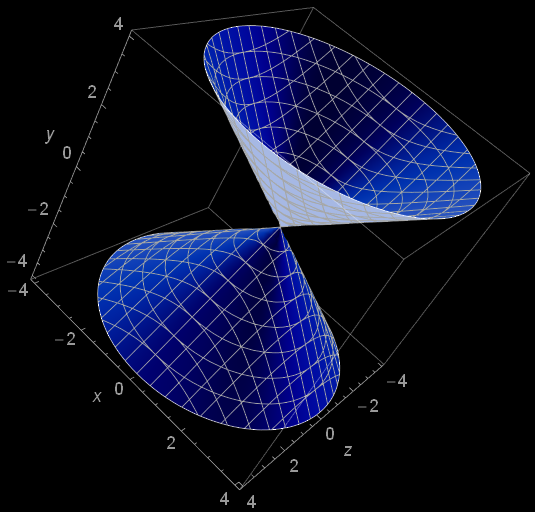
\includegraphics[width=\marginparwidth]{3d_cone.png}
    \caption{A 3D cone in $\mathbb{R}^3$, from WolframAlpha}\label{fig:a_3d_cone_in_r_3_}
  \end{marginfigure}
  However, this is not a manifold: if we assume that a ball arounnd the origin
  is homeomorphic to $\mathbb{R}^2$, then by removing the point at the origin
  in the cone, the cone becomes two disconnected components, but the ball in
  $\mathbb{R}^2$ homeomorphic to the aforementioned ball is still connected.
\end{eg}

\begin{note}
  An open subset of a manifold is a manifold, by restriction.
\end{note}

\subsection{The $1$-Sphere $S^1$}%
\label{sub:the_1_sphere_s_1_}
% subsection the_1_sphere_s_1_

From \cref{eg:basis_of_r_n}, we have
\begin{itemize}
  \item $[0, 1) \simeq [0, \infty)$ is a manifold with boundary;
  \item $(0, 1) \simeq \mathbb{R}$ is a manifold; and
  \item $[0, 1]$ is a manifold with boundary.
\end{itemize}

\begin{eg}[$S^1$ is a manifold]
  Consider the function $f : [0, 2 \pi) \to e^{i \theta}$. The image of $f$ is
  \begin{figure}[ht]
    \centering
    \begin{tikzpicture}
      \draw[{Bracket[length=5pt,width=20pt]}-{Arc Barb[length=5pt,width=20pt]}] (0, 0) arc(0:360:1.5) node[circle,fill,inner sep=1pt] {};
    \end{tikzpicture}
    \caption{$S^1$ as a manifold}
    \label{fig:s_1_as_a_manifold}
  \end{figure}
  Consider the following two functions $(0, 2\pi) \to \mathbb{C}^2$ by
  \begin{gather*}
    \theta_1 \to e^{i \theta_1} \text{ and } \theta_2 \to e^{i \theta_2 + \pi},
  \end{gather*}
  which gives us the graphs:
  \begin{figure}[ht]
    \centering
    \begin{tikzpicture}
      \draw (0, 0) circle(1);
      \node[circle,draw,inner sep=1.5pt] at (1, 0) {};
      \draw (3, 0) circle(1);
      \node[circle,draw,inner sep=1.5pt] at (2, 0) {};
    \end{tikzpicture}
    \caption{Basis for $S^1$}
    \label{fig:basis_for__s_1_}
  \end{figure}

  \noindent
  respectively. Note that the image of both these functions are not compact.
  Regardless, this gives us a basis for $S^1$, which we notice is countable,
  Hausdorff, and locally homeomorphic to $\mathbb{R}^2$.
\end{eg}

\begin{thm}[$1$-Dimensional Manifolds Determined by Its Compactness]\label{thm:_1_dimensional_manifolds_determined_by_its_compactness}
  Let $M$ be a connected component of a $1$-dimensional manifold. Then either
  \begin{enumerate}
    \item $M$ is compact, in which case if it is
      \begin{itemize}
        \item without a boundary, then $M$ is homeomorphic to $S^1$.
        \item with a boundary, then $M$ is homeomorphic to $[0, 1]$.
      \end{itemize}
    \item $M$ is not compact, in which case if it is
      \begin{itemize}
        \item without a boundary, then $M$ is homeomorphic to $[0, 1)$.
        \item with a boundary, then $M$ is homeomorphic to $(0, 1)$.
      \end{itemize}
  \end{enumerate}
\end{thm}

% subsection the_1_sphere_s_1_ (end)

% section manifolds_continued (end)

% chapter lecture_5_jan_16th (end)

\chapter{Lecture 6 Jan 18th}%
\label{chp:lecture_6_jan_18th}
% chapter lecture_6_jan_18th

\section{Manifolds (Continued 2)}%
\label{sec:manifolds_continued_2}
% section manifolds_continued_2

\subsection{The $1$-Sphere $S^1$ (Continued)}%
\label{sub:the_1_sphere_s_1_continued}
% subsection the_1_sphere_s_1_continued

\paragraph{Set theoretic view of $S^1$}
We showed that $S^1$ is a manifold. We can, in fact, set theoretically, look
at $S^1$ as $A = [0, 1]$ glued at the endpoints, i.e. we \hlnotea{identify}
the points $0$ and $1$ as `the same', and label this notion as $0 \sim 1$.

\paragraph{Topological view of $S^1$}
Topologically, for $0 \sim 1$ in $A$, we can construct an open set around the
point such that the open set is properly contained in $A$.

\begin{figure}[ht]
  \centering
  \begin{tikzpicture}
    \draw[{Bracket[length=5pt,width=15pt]}-{Bracket[length=5pt,width=15pt]}] (-2, 0) -- (2, 0);
    \draw[-{Arc Barb[length=5pt,width=15pt]},be-blue] (-2,0) -- (-1,0);
    \draw[{Arc Barb[length=5pt,width=15pt]}-,be-blue] (1,0) -- (2,0);
    \node[circle,fill=be-blue,inner sep=1.5pt] at (-2, 0) {};
    \node[circle,fill=be-blue,inner sep=1.5pt] at (2, 0) {};
  \end{tikzpicture}
  \caption{Topological representation of $A$}
  \label{fig:topological_representation_of_a}
\end{figure}

But how can we describe this notion mathematically so?

\newthought{Consider} the real line as follows:

\begin{figure*}[ht]
  \centering
  \begin{tikzpicture}[scale=1.5]
    \draw[->] (-5, 0) -- (5, 0);
    \foreach \x in {-4,-3,...,4} {
      \draw[dashed,color=be-blue] (\x,0.5) -- (\x,-0.5);
      \node[circle,fill,inner sep=2pt,label={270:{$\x$}}] at (\x, 0) {};
      \node[label={[label distance=1]above:{$T^{\x}(a)$}}] at (\x + 0.3, 0) {$( \times )$};
      \node at (\x + 0.7, 0) {$\blacktriangle$};
    }
  \end{tikzpicture}
  \caption{Breaking down the real line into parts}
  \label{fig:breaking_down_the_real_line_into_parts}
\end{figure*}

Let's define $T : \mathbb{R} \to \mathbb{R}$ such that $x \mapsto x + 1$. Clearly
so, $T$ is bijective and, in particular, has an inverse $x \mapsto x - 1$.

Notice that within each interval $[x, x + 1]$, we can find a $\times$ and
$\blacktriangle$ at the same distance from $x$. Also, notice that we can use the
same radius for $\times$ such that the open ball around $\times$ sits in $[x, x + 1]$
for each $x \in \mathbb{Z}$.

Thus, instead of studying the entire real line at once, we can reduce our attention
only to $[0, 1]$, and simply scale the interval with a `scalar multiplication' to
get to wherever we want on the real line.

Now let
\begin{equation*}
  G := \left\{ T^k \mmid k \in \mathbb{Z} \right\},
\end{equation*}
which is evidently a \hldefn{group}. Furthermore, every element in $G$ is a
homeomorphism to $\mathbb{R}$. Let $G$ \hldefn{act on} $\mathbb{R}$, and for
$a \in \mathbb{R}$, consider the \hldefn{orbit} of $a$, which is denoted as
\begin{equation*}
  G \cdot a := \left\{ T^k (a) \mmid k \in \mathbb{Z} \right\}.
\end{equation*}
Then
\begin{equation*}
  S^1 \simeq \text{ the space of all orbits of } G \text{ acting on } \mathbb{R} =: \mathbb{R} / G,
\end{equation*}
where $\simeq$ represents \hyperref[defn:homeomorphism]{homeomorphism}.
\sidenote{$\mathbb{R} / G$ is the \hldefn{quotient space} of $\mathbb{R}$ over $G$.}
Also, notice that here, $G$ is effectively $\mathbb{Z}$.

This realization implies the existence of some topology on $S^1$.

\newthought{Thus far}, we have seen that we may look at $S^1$
\begin{itemize}
  \item set theoretically: as $A = [0, 1]$ with glued endpoints; and
  \item topologically: as $\mathbb{R} \setminus \mathbb{Z}$.
\end{itemize}

\paragraph{$S^1$ as a topological group}
Since $\mathbb{C} \simeq \mathbb{R}^2$, we may think of $S^1$ as a
sphere on the complex plane.
\begin{figure*}[ht]
  \centering
  \begin{tikzpicture}[scale=1.3]
    \draw[->] (-2,0) -- (2, 0);
    \draw[->] (0,-2) -- (0, 2);
    \draw (0, 0) circle(1);
    \draw (0, 0) -- (0.7071067811865475244,0.7071067811865475244)
      node[circle,fill,inner sep=1pt,label={45:{$z_1 = e^{i \theta_1}$}}] {};
    \draw (0, 0) -- (-0.7071067811865475244,0.7071067811865475244)
      node[circle,fill,inner sep=1pt,label={135:{$z_2 = e^{i \theta_2}$}}] {};
    \draw[dashed] (0, 0) -- (-0.7071067811865475244,-0.7071067811865475244)
      node[circle,fill,inner sep=1pt,label={225:{$z_1 z_2 = e^{i ( \theta_1 + \theta_2 )}$}}] {};
    \node[scale=1.3,right] at (1, 1.5) {$S^1 = \left\{ z \in \mathbb{C} \mid \abs{ z } = 1 \right\} = \left\{ e^{i \theta} \mid \theta \in \mathbb{R} \right\}$};
  \end{tikzpicture}
  \caption{$S^1$ on the complex plane}
  \label{fig:_s_1_on_the_complex_plane}
\end{figure*}
We see that this `group' takes on the operation of adding the indices
of the exponents. Thus $G = ( S^1, \cdot )$. Notice that $G$ is indeed
a group equipped with said operation, and for each $z_1 \in G$, there
exists $z_1^{-1} = \frac{1}{z_1} \in G$ such that
$z_1 \cdot \frac{1}{z_1} = 1$.

Furthermore, the function
\begin{gather*}
  \iota : S^1 \to S^1 \text{ given by } z \mapsto \frac{1}{z} \\
  \text{ which is } e^{i \theta} \mapsto e^{- i \theta}
\end{gather*}
is continuous.

Also, the function
\begin{equation*}
  P : S^1 \times S^1 \to S^1 \text{ given by } (z_1, z_2) \mapsto z_1 z_2
\end{equation*}
is continuous.

\begin{defn}[Topological Group]\index{Topological Group}\label{defn:topological_group}
  If $G$ is a group, and functions $\iota$ and $P$ as defined above,
  if both $\iota$ and $P$ are continuous, then we say that $G$ is a
  \hlnoteb{topological group}.
\end{defn}

\paragraph{$S^1$ as a moduli space}

\begin{defn}[Moduli Space]\index{Moduli Space}\label{defn:moduli_space}
  A \hlnoteb{moduli space} is the space of all lines passing through
  the origin.
\end{defn}

On $\mathbb{R}^2$, we have
\begin{figure}[ht]
  \centering
  \begin{tikzpicture}
    \draw[->] (-2, 0) -- (2, 0);
    \draw[->] (0, -2) -- (0, 2);
    \draw (0, 0) circle(1);

    \clip (-2, -2) rectangle (2, 2);
    \foreach \m in {-3,-2.5,...,3} {
      \draw[color=be-blue] plot ({\x}, {\m * \x});
    }
  \end{tikzpicture}
  \caption{The moduli space on $\mathbb{R}^2$}
  \label{fig:the_moduli_space_on_r_2_}
\end{figure}

First, how can we understand `closeness' in a moduli space?
We can actually look at the difference in the radians of each
line, or really just $x / 360$ and compare the $x$'s.

Also, notice that each line passes through $S^1$ twice. We can
indeed avoid this problem by shifting $S^1$ to one side, as
shown in \cref{fig:shifted_s_1_for_the_moduli_space}.
\begin{marginfigure}
  \centering
  \begin{tikzpicture}
    \draw[->] (-1, 0) -- (3, 0);
    \draw[->] (0, -2) -- (0, 2);
    \draw (1, 0) circle(1);

    \clip (-2, -2) rectangle (3, 2);
    \foreach \m in {-3,-2.5,...,3} {
      \draw[color=be-blue] plot ({\x}, {\m * \x});
    }
  \end{tikzpicture}
  \caption{Shifted $S^1$ for the moduli space}\label{fig:shifted_s_1_for_the_moduli_space}
\end{marginfigure}
Now each line intersects $S^1$ at the origin and another
point on $S^1$, and this intersection is in fact unique.

\subsubsection{The space of $S^1 \times S^1$}%
\label{ssub:the_space_of_s_1_times_s_1_}
% subsubsection the_space_of_s_1_times_s_1_

Observe that the product of two manifolds is a manifold
\sidenote{This is called a \hldefn{product space}.}.

\newthought{Consider} using the set theoretical viewpoint,
with credits to \hlnotea{Felix Klein}, the following figure
\begin{figure*}[ht]
  \centering
  \begin{tikzpicture}
    \draw[{Bracket[length=5pt,width=15pt]}-{Bracket[length=5pt,width=15pt]}] (0, 0) -- (2, 0);
    \draw[{Bracket[length=5pt,width=15pt]}-{Bracket[length=5pt,width=15pt]}] (0, 0) -- (0, 2);
    \node[circle,fill,inner sep=2pt] at (0, 0) {};
    \node[circle,fill,inner sep=2pt] at (2, 0) {};
    \draw (0, 2) -- (2, 2) -- (2, 0);
    \node at (1, 0) {$>$};
    \node at (1, 2) {$>$};
    \node[rotate=90] at (0, 1) {$>>$};
    \node[rotate=90] at (2, 1) {$>>$};

    \node at (3, 1) {$\leadsto$};

    \draw (4, 0.5) arc(-90:90:0.25 and 0.5)
      node[midway,rotate=90] {$>>$};
    \draw (4, 0.5) arc(-90:-270:0.25 and 0.5);
    \draw (4, 1.5) -- (6, 1.5) node[midway] {$>$};
    \draw (4, 0.5) -- (6, 0.5) node[midway] {$>$};
    \draw (6, 0.5) arc(-90:90:0.25 and 0.5)
      node[midway,rotate=90] {$>>$};
    \draw[dashed] (6, 0.5) arc(-90:-270:0.25 and 0.5);

    \node at (7, 1) {$\leadsto$};

    \draw (8.3,1) to[bend left] (8.8,1);
    \draw (8.1,1.1) to[bend right] (9,1.1);
    \draw[rotate=0] (8.5,1) ellipse (30pt and 15pt);
  \end{tikzpicture}
  \caption{$S^1 \times S^1$ becomes a cylinder by identifying the edges}
  \label{fig:_s_1_times_s_1_becomes_a_cylinder_by_identifying_the_edges}
\end{figure*}
By joining the sides with $>$, where we identify the endpoints,
we can go from the figure introduced by Klein to a cylinder. Then
by identifying the sides with $>>$, we get a \hldefn{torus}.

\newthought{Now on} a Cartesian plane, observe that
\begin{figure*}[ht]
  \centering
  \begin{tikzpicture}
    \foreach \z in {-2,-1,...,3} {
      \draw[dashed,color=be-blue!50!dark] (\z, -2) -- (\z, 2);
    }
    \draw[->] (-2, 0) -- (3, 0);
    \draw[->] (0, -2) -- (0, 2);
    \draw (0, 0) -- (1, 0) -- (1, 1) -- (0, 1) --cycle;
    \node at (0.5, 0) {$>$};
    \node at (0.5, 1) {$>$};
    \node[rotate=90] at (0, 0.5) {$>>$};
    \node[rotate=90] at (1, 0.5) {$>>$};

    \draw[->] (2, 1) to[bend left] (5,1);

    \draw (4, -0.5) arc(-90:90:0.25 and 0.5)
      node[midway,rotate=90] {$>>$};
    \draw (4, -0.5) arc(-90:-270:0.25 and 0.5);
    \draw (4, 0.5) -- (6, 0.5) node[midway] {$>$};
    \draw (4, -0.5) -- (6, -0.5) node[midway] {$>$};
    \draw (6, -0.5) arc(-90:90:0.25 and 0.5)
      node[midway,rotate=90] {$>>$};
    \draw[dashed] (6, -0.5) arc(-90:-270:0.25 and 0.5);

    \node at (8, 0) {$\simeq \mathbb{R}^2 / G$};
  \end{tikzpicture}
  \caption{Klein's figure on a Cartesian plane to a cylinder}
  \label{fig:klein_s_figure_on_a_cartesian_plane_to_a_cylinder}
\end{figure*}

\noindent
where we define $G = \left\{ T^k \mmid k \in \mathbb{Z} \right\}$ as before,
for $T ((x, y)) = (x + 1, y)$. Now on a similar note, define
$R : \mathbb{R} \to \mathbb{R}$ by $R((x, y)) = (x, y + 1)$. Then let
$G_2 = \left\{ R^k \mmid k \in \mathbb{Z} \right\}$. Thus
\begin{equation*}
  \mathbb{R}^2 / G \oplus G_2 \simeq \mathbb{R}^2 / \mathbb{Z} \oplus \mathbb{Z}.
\end{equation*}

% subsubsection the_space_of_s_1_times_s_1_ (end)

% subsection the_1_sphere_s_1_continued (end)

% section manifolds_continued_2 (end)

% chapter lecture_6_jan_18th (end)

\chapter{Lecture 7 Jan 21st}%
\label{chp:lecture_7_jan_21st}
% chapter lecture_7_jan_21st

\section{Manifolds (Continued 3)}%
\label{sec:manifolds_continued_3}
% section manifolds_continued_3

\subsection{\texorpdfstring{$2$}{2}-dimensional Manifolds}%
\label{sub:_2_dimensional_manifolds}
% subsection _2_dimensional_manifolds

\begin{eg}\label{eg:2_sphere_as_a_manifold}
  $S^2$ is a $2$-dimensional manifold (w/o boundary).
  \begin{marginfigure}
    \centering
    \begin{tikzpicture}
      \pgfmathsetmacro\rad{1};
      \draw (0, 0, 0) circle(\rad);
      \shade[ball color=be-blue!70!dark,opacity=0.5] (0, 0, 0) circle(\rad);
      \draw[opacity=0.5] (-\rad,0,0) arc (180:360:{\rad} and {\rad/2});
      \draw[dashed,opacity=0.5] (-\rad,0,0) arc (180:0:{\rad} and {\rad/2});
      \draw[opacity=0.5] (0,\rad,0) arc (90:270:{\rad/2} and \rad);
      \draw[dashed,opacity=0.5] (0,\rad,0) arc (90:-90:{\rad/2} and \rad);

      \fill[color=be-red,opacity=0.3] (-{\rad}, 0, 0) arc (180:360:{\rad}) -- ({\rad}, 0, 0) arc (360:180:{\rad} and {\rad/2});
      \fill[color=be-red,opacity=0.2] (-{\rad}, 0, 0) arc (180:0:{\rad} and {\rad/2}) -- ({\rad}, 0, 0) arc (360:180:{\rad} and {\rad/2});

      % the axes
      \draw[dashed] (-2, 0, 0) -- (0, 0, 0);
      \draw[dashed] (0, -2, 0) -- (0, 0, 0);
      \draw[dashed] (0, 0, -2) -- (0, 0, 0);
      \draw[-latex'] (0, 0, 0) -- (2, 0, 0) node[right] {$y$};
      \draw[-latex'] (0, 0, 0) -- (0, 2, 0) node[above] {$z$};
      \draw[-latex'] (0, 0, 0) -- (0, 0, 2) node[below,left] {$x$};
    \end{tikzpicture}
    \caption{The $2$-sphere $S^2$}
    \label{fig:the_2_sphere_s_2_}
  \end{marginfigure}
  Note that we may `cover' this sphere by the function $f_{-} : \mathbb{D} \subseteq \mathbb{R}^2 \to \mathbb{R}$,
  where $\mathbb{D}$ is the unit disc in $\mathbb{R}^2$, and $f_{-}$ is given by
  \begin{equation*}
    (x, y) \mapsto - \sqrt{1 - (x^2 + y^2)}.
  \end{equation*}
  We see that $f_{-}$ is a chart for the lower hemisphere for \cref{fig:the_2_sphere_s_2_}, shaded red.
  We can indeed cover the entire $2$-sphere with similar hemispheres in different orientations: consider
  \begin{gather*}
    f_+ (x, y) = \sqrt{ 1 - x^2 - y^2 } \\
    g_+ (x, z) = \sqrt{ 1 - x^2 - z^2 } \\
    g_- (x, z) = - \sqrt{ 1 - x^2 - z^2 } \\
    h_+ (y, z) = \sqrt{ 1 - y^2 - z^2 } \\
    h_- (y, z) = - \sqrt{ 1 - y^2 - z^2 },
  \end{gather*}
  which represent the upper hemisphere, eastern hemisphere, western hemisphere, front hemisphere,
  and back hemisphere, respectively.
\end{eg}

We have the following general observation: let $f : \mathcal{U} \subseteq \mathbb{R}^n \to \mathbb{R}$
be a real-valued continuous function. Then $\Gamma(f)$ is \hlnotea{parameterized} using $f$, i.e. $f$
constructs the chart $\Gamma(f)$.

We have not explicitly defined what $\Gamma(f)$ is, but it is recorded
in \href{https://tex.japorized.ink/PMATH733/classnotes.pdf\#page.32}{PMATH 733}, but we shall provide a
short definition here for reference: the \hldefn{graph} $\Gamma(f)$ of the function $f$ is defined as
\begin{equation*}
  \Gamma(f) := \left\{ (x_1, \ldots, x_n, y) \mmid f(x_1, \ldots, x_n) = y \right\}.
\end{equation*}

It is interesting to note that $\Gamma(f)$ is homeomorphic to $\mathcal{U}$. Consider the function
\begin{equation*}
  \Phi : \mathcal{U} \to \Gamma(F) \text{ given by } \Phi(x_1, \ldots, x_n) = (x_1, \ldots, x_n, f(x_1, \ldots, x_n)).
\end{equation*}
It is clear that $\Phi$ is continuous since each of its components are continuous. However, it is not
as easy to find a continuous map to go from $\Gamma(f)$ to $\mathcal{U}$.

\begin{defn}[Projection]\index{Projection}\label{defn:projection}
  We define function $\pi_{n + 1} : \Gamma(f) \to \mathcal{U}$ by
  \begin{equation*}
    \pi_{n + 1}(x_1, \ldots, x_n, y) = (x_1, \ldots, x_n),
  \end{equation*}
  which is called a \hlnoteb{projection}.
\end{defn}

\begin{note}
  \begin{enumerate}
    \item In A1, we showed that $\pi_{n + 1}$ is continuous.
    \item Furthermore, $\pi_{n + 1}$ is injective.
    \item Thus, we observe that
      \begin{equation*}
        \pi_{n + 1} \circ \Phi(x_1, \ldots, x_n) = (x_1, \ldots, x_n) = id_{n + 1}(x_1, \ldots, x_n).
      \end{equation*}
  \end{enumerate}
\end{note}

\begin{eg}
  Consider the following figure:
  \begin{figure}[ht]
    \centering
    \begin{tikzpicture}
      \draw (0, 0, 0) circle(2);
      \shade[ball color=be-blue!70!dark,opacity=0.5] (0, 0, 0) circle(2);
      \draw[opacity=0.5] (-2,0,0) arc (180:360:2 and 1);
      \draw[dashed,opacity=0.5] (-2,0,0) arc (180:0:2 and 1);
      \draw[opacity=0.5] (0,2,0) arc (90:270:1 and 2);
      \draw[dashed,opacity=0.5] (0,2,0) arc (90:-90:1 and 2);
      \draw (0, 0, 0) circle(2);

      % Stereographic projection
      \node[draw,circle,color=be-red,fill,inner sep=1.5pt,pin={[pin edge=latex'-, pin distance=5pt]45:{$N$, the north pole}}] at (0, 2, 0) {};
      \node[draw,circle,color=be-red,fill,inner sep=1.5pt,pin={[pin edge={latex'-}, pin distance=40pt]30:{$p$}}] at (1.5, 1, 0.5) {};
      \node[draw,circle,color=be-red,fill,inner sep=1.5pt,pin={[pin edge=latex'-, pin distance=20pt]245:{$p'$}}] at (3, 0, 1) {};
      \draw[thick,be-red] (0, 2, 0) -- (1.5,1,0.5) -- (3, 0, 1);

      \draw[dashed] (3, 0, 1) -- (0, 0, 0);
      \draw[dashed] (3, 0, 0) -- (3, 0, 1) -- (0, 0, 1);
      \draw[dashed] (0, 0, 0) -- (1.5, 1, 0.5) -- (1.5, 0, 0.5) -- (0, 0, 0.5);
      \draw[dashed] (1.5, 0, 0) -- (1.5, 0, 0.5);

      % the axes
      \draw[dashed] (-3, 0, 0) -- (0, 0, 0);
      \draw[dashed] (0, -3, 0) -- (0, 0, 0);
      \draw[dashed] (0, 0, -3) -- (0, 0, 0);
      \draw[-latex'] (0, 0, 0) -- (3.5, 0, 0) node[right] {$y$};
      \draw[-latex'] (0, 0, 0) -- (0, 3, 0) node[above] {$z$};
      \draw[-latex'] (0, 0, 0) -- (0, 0, 3) node[below,left] {$x$};
    \end{tikzpicture}
    \caption{Stereographic Projection}
    \label{fig:stereographic_projection}
  \end{figure}

  We define the \hldefn{stereographic projection} by
  \begin{equation*}
    \Sigma(p) = p'.
  \end{equation*}
\end{eg}

% subsection _2_dimensional_manifolds (end)

\subsection{\texorpdfstring{$n$}{n}-spheres}%
\label{sub:_n_spheres}
% subsection _n_spheres

We can now extend the notion we saw in \cref{eg:2_sphere_as_a_manifold} to higher dimensional
manifolds. In particular, we want to be able to `glue' the boundaries of the hemispheres, as
shown in \cref{fig:glueing_two_hemispheres}.

\begin{marginfigure}
  \centering
  \begin{tikzpicture}
    \draw[dashed] (-2, 1, 0) -- (-2, -1.5, 0);
    \draw[dashed] (2, 1, 0) -- (2, -1.5, 0);
    \draw[dashed] (-1.5, 1, -2.3) -- (-1.5, -1.5, -2.3);
    \draw[dashed] (0, 1, -2.3) -- (0, -1.5, -2.3);
    \draw[dashed] (1, 1, 2.6) -- (1, -1.5, 2.6);

    \draw[dashed] (-2, 1, 0) arc (180:0:2 and 1);
    \draw[fill=be-red,fill opacity=0.5] (-2, 1, 0) arc (180:360:2 and 1) -- (2, 1, 0) arc (0:180:2);

    \draw[fill=light,fill opacity=0.5] (-2, -1.5, 0) arc (180:360:2) -- (2, -1.5, 0) arc (0:180:2 and 1) -- (-2, -1.5, 0) arc (180:360:2 and 1);

    \begin{scope}
      \clip (-2, 1, 0) arc (180:360:2 and 1) -- (2, 1, 0) arc (0:180:2);
      \draw[fill=dark!70!light] (1, 1, 2.6) circle(0.5);
    \end{scope}
    \node[draw,circle,fill] at (1, 1, 2.6) {};

    \begin{scope}
      \clip (-2, -1.5, 0) arc (180:360:2) -- (2, -1.5, 0) arc (360:180:2 and 1);
      \draw[fill=dark!70!light] (1, -1.5, 2.6) circle(0.5);
    \end{scope}
    \node[draw,circle,fill] at (1, -1.5, 2.6) {};
  \end{tikzpicture}
  \caption{Glueing two hemispheres}\label{fig:glueing_two_hemispheres}
\end{marginfigure}
\marginnote{I was definitely not trying to make a Pokeball.}

In a more mathematical sense, we are identifying the lower and upper boundaries of the upper
and lower hemisphere, respectively, i.e. we identify
\begin{equation*}
  S^n = \bar{\mathbb{B}}^n \times \{ 0 \} \cup \bar{\mathbb{B}}^n \times \{ 1 \},
\end{equation*}
where the $\{ 0 \}$ and $\{ 1 \}$ represent the upper and lower hemispheres, respectively. We
may also write this as
\begin{equation*}
  x \in \partial \bar{\mathbb{B}}^n : (x, 0) \sim (x, 1).
\end{equation*}

This calls for the notion of an equivalence class. Recall that an \hldefn{equivalence relation}
on a set $A$ is a relation between elements such that
\begin{enumerate}
  \item (reflexity) $x \sim x$;
  \item (symmetry) $x \sim y \iff y \sim x$; and
  \item (transitivity) $x \sim y \, \land \, y \sim z \implies x \sim z$,
\end{enumerate}
where $\sim$ is our equivalence relation.

Equivalence relations give rise to the notion of \hldefn{equivalence classes}, where we define
an equivalence class as
\begin{equation*}
  [\beta] := \{ \alpha \in A \mid \beta \sim \alpha \}.
\end{equation*}
In this course, we shall sometimes denote equivalence classes in the form of $A_\beta$. Notice
that
\begin{equation*}
  A = \coprod\limits_{\beta \in B} A_\beta,
\end{equation*}
where $B \subseteq A$.

\newthought{This begs the question}: do the set of equivalence classes retain the topology of
the space?

Here, we look into \hldefn{quotient topology}. Let $A^*$ be the space of equivalence classes,
and let's assume that $A$ is endowed with a topology. Consider the function
\begin{equation*}
  \pi : A \to A^* \text{ given by } a \mapsto [a]_{\sim},
\end{equation*}
where $\sim$ is the equivalence relation, and $[a]_{\sim}$ is the equivalence class that $a$
belongs to\sidenote{Note that the function is well-defined as the equivalence classes are
disjoint.}.

\begin{figure}[ht]
  \centering
  \begin{tikzcd}
    A \arrow[dd, "\pi"'] \arrow[rrdd, "g"] &  &  \\
     &  &  \\
    A^* \arrow[rr, "\tilde{g}"'] &  & Z
  \end{tikzcd}
  \caption{Relationship of $A$, $A^*$ and $Z$}
  \label{fig:relationship_of_a_a_and_z_}
\end{figure}

Consider an arbitrary space $Z$ that is also endowed with a topology, such that
$\exists g : A \to Z$ that is continuous, such that $g$ is constant on each of the equivalence
classes of $A$, that is, if $a \sim b$, then $g(a) = g(b)$.

Then $\tilde{g}$ is a well-defined function induced on $A^*$: we have that
\begin{equation*}
  \tilde{g}(\pi(a)) = g(a).
\end{equation*}

We want to endow $A^*$ with a topology such that $\tilde{g}$ will be continuous. However,
\begin{itemize}
  \item if $A^*$ is too `fine', then $\pi$ may not be continuous; and
  \item if $A^*$ is too `course', then $\tilde{g}$ may not be continuous.
\end{itemize}
We need to strike a balance in the fineness of the topology of $A^*$ to make sure that both
$\pi$ and $\tilde{g}$ are continuous.

\begin{defn}[Strongly Continuous]\index{Strongly Continuous}\label{defn:strongly_continuous}
  Let $\mathcal{V} \subseteq A^*$. $\mathcal{V}$ is open iff $\exists \mathcal{U} \subseteq A$
  such that $\pi(\mathcal{U}) = \mathcal{V}$. We say that $\pi$ is \hlnoteb{strongly continuous}.
\end{defn}

\begin{warning}
  $\pi$ may not be an open map!
\end{warning}

% subsection _n_spheres (end)

% section manifolds_continued_3 (end)

% chapter lecture_7_jan_21st (end)

\chapter{Lecture 8 Jan 23rd}%
\label{chp:lecture_8_jan_23rd}
% chapter lecture_8_jan_23rd

\section{Quotient Spaces}%
\label{sec:quotient_spaces}
% section quotient_spaces

With the topology that we last introduced for $A^*$, $g$ is continuous iff $\tilde{f}$ is continuous.
\marginnote{This way of constructing a quotient space is intuitive, ring theoretically.}
However, this is a rather cumbersome way to construct a quotient space. In particular, how do we know
what equivalence class should we choose?

\marginnote{
\begin{ex}
  Let $\pi : X \to Y$ be any map. For a subset $U \subseteq X$, show that TFAE.
  \begin{enumerate}
    \item $U$ is saturated.
    \item $U = \pi^{-1}(q(U))$.
    \item $U$ is a union of fibres.
    \item If $x \in U$, then every point $x' \in X$ such that $q(x) = q(x')$ is also in $U$.
  \end{enumerate}
\end{ex}
}
\begin{defn}[Saturated]\index{Saturated}\label{defn:saturated}
  We say that a subset $S \subseteq A$ is \hlnoteb{saturated} (wrt $\pi$) provided that it is has
  a \hlimpo{non-empty intersection} with a fibre $\pi^{-1}(\{ q \})$, where $q \in A^*$, then
  $S \supseteq \pi^{-1}(\{ q \})$.
\end{defn}

\begin{note}
  This definition is equivalent to saying that $\pi^{-1} \circ \pi (S) = S$.
\end{note}

With this definition, we may restate the definition of a quotient map in a clearer way.

\begin{defn}[Quotient Map]\index{Quotient Map}\label{defn:quotient_map}
  A map $g : X \to Y$ is called a \hlnoteb{quotient map} if it sends saturated open subsets of $X$
  to open subsets of $Y$.
\end{defn}

\begin{eg}
  Let $g : X \to Y$ be surjective. We can define an equivalence relation on $X$ by setting
  $x_1 \sim x_2$ iff $g(x_1) = g(x_2)$, i.e. $x_1$ and $x_2$ belong to the same fibre.
\end{eg}

\begin{eg}
  Let $\bar{\mathbb{B}}^2$ be the closed unit disk in $\mathbb{R}^2$, and let $\sim$ be the
  equivalence relation on $\bar{\mathbb{B}}^2$ defined by $(x, y) \sim (-x, y)$ for all $(x, y)
  \in \partial \bar{\mathbb{B}}^2$ (See \cref{fig:a_quotient_of_b_2}).
  \begin{marginfigure}
    \centering
    \begin{tikzpicture}
      \draw[fill=be-blue!30!dark] (0, 0) circle(1);
      \draw[midarrow] (0, 1) arc(90:270:1);
      \draw[midarrow] (0, 1) arc(90:-90:1);
      \node[draw,circle,fill,inner sep=1pt] at (0, 1) {};
      \node[draw,circle,fill,inner sep=1pt] at (0, -1) {};
    \end{tikzpicture}
    \caption{A quotient of $\bar{\mathbb{B}}^2$}\label{fig:a_quotient_of_b_2}
  \end{marginfigure}
  We can think of this space as one that is obtained from $\mathbb{B}^2$ by ``pasting'' the
  left half of the boundary to the right half. It is not difficult to imagine this transformation
  and notice that we can `continuously morph' $\mathbb{B}^2$ under this equivalence relation into
  $S^2$. We shall prove much later on that this is indeed the case.

  The above process is also called `collapsing $\partial \mathbb{B}^2$ to a point'.
\end{eg}

\begin{eg}
  Define an equivalence relation on the square $I \times I$ by setting $(x, 0) \sim (x, 1)$ for
  all $x \in I$, and $(0, y) \sim (1, y)$ for all $y \in I$ (See
  \cref{fig:a_quotient_of_i_times_i_}).
  \begin{marginfigure}
    \centering
    \begin{tikzpicture}
      \draw[fill=be-blue!30!dark] (-1, 1) -- (-1, -1) -- (1, -1) -- (1, 1) --cycle;
      \draw[midarrow={>>}{0.5}] (-1, 1) -- (-1, -1);
      \draw[midarrow={>>}{0.5}] (1, 1) -- (1, -1);
      \draw[midarrow={>}{0.5}] (1, 1) -- (-1, 1);
      \draw[midarrow={>}{0.5}] (1, -1) -- (-1, -1);
    \end{tikzpicture}
    \caption{A quotient of $I \times I$}\label{fig:a_quotient_of_i_times_i_}
  \end{marginfigure}
\end{eg}

\begin{eg}
  Define $\mathbb{P}^n$, the \hldefn{real projective space of dimension $n$}, to be the set of
  $1$-dimensional linear subpaces (lines through the origin) in $\mathbb{R}^{n + 1}$. There
  exists a map $q : \mathbb{R}^{n + 1} \setminus \{ 0 \} \to \mathbb{P}^n$, defined by sending
  a point $x$ to its span. We apply the quotient topology with respect to $q$ on $\mathbb{P}^2$.
  The $2$-dimensional projective space $\mathbb{P}^2$ is usually called the \hldefn{projective
  plane}.
\end{eg}

\begin{eg}
  Let $X$ be a topological space, the quotient $(X \times I) / (X \times \{ 0 \})$ obtained from
  the ``cylinder'' $X \times I$ by collapsing one end to a point is called the \hldefn{cone} on
  $X$. For instance, if $X = S^1$ and $I = (0, 1)$, then taking the quotient
  $(S^1 \times (0, 1)/(S^1 \times \{ 0 \})$ is exactly the process shown in
  \cref{fig:cone_of_s_1_}.
  \begin{marginfigure}
    \centering
    \begin{tikzpicture}
      \draw (-1, 1) -- (-1, -2) arc(180:360:1 and 0.5) -- (1, -2) --
        (1, 1) arc(0:180:1 and 0.5) -- (-1,1) arc(180:360:1 and 0.5);
      \draw[dashed] (-1, -2) arc(180:0:1 and 0.5);

      \node[rotate=-90,scale=1.5] at (0, -3) {$\leadsto$};

      \draw (0, -4) -- (-1, -7) arc(180:360:1 and 0.5) -- (1, -7) -- cycle;
      \draw[dashed] (-1, -7) arc(180:0:1 and 0.5);
    \end{tikzpicture}
    \caption{Cone of $S^1$}\label{fig:cone_of_s_1_}
  \end{marginfigure}
\end{eg}

\begin{eg}[Wedge sum of Manifolds]\label{eg:wedge_sum_of_manifolds}
  Let $M_1$ and $M_2$ be two manifolds. We define the \hldefn{wedge sum} of $M_1$ and $M_2$ as
  \begin{equation*}
    M_1 \lor M_2 := (M_1 \cup M_2) / p_1 \sim p_2,
  \end{equation*}
  where $p_1 \in M_1$ and $p_2 \in M_2$. The wedge sum is also sometimes called the
  \hldefn{one-point union}.
  \begin{marginfigure}
    \centering
    \begin{tikzpicture}
      \draw[latex-latex] (-1, 0) -- (1, 0);
      \draw[latex-latex] (0, -1) -- (0, 1);
      \node[draw,circle,fill,inner sep=1.5pt] at (0, 0) {};
    \end{tikzpicture}
    \caption{Wedge sum of two lines.}\label{fig:wedge_sum_of_two_lines}
  \end{marginfigure}
  \begin{marginfigure}
    \centering
    \begin{tikzpicture}
      \draw (0, 1) circle(1);
      \draw (0, -1) circle(1);
      \node[draw,circle,fill,inner sep=1.5pt] at (0, 0) {};
    \end{tikzpicture}
    \caption{Wedge sum of two circles.}\label{fig:wedge_sum_of_two_circles}
  \end{marginfigure}
  For instance, the wedge sum of $\mathbb{R} \wedge \mathbb{R}$ is homeomorphic to the union
  of the $x$-axis and $y$-axis on a Cartesian plane (cf \cref{fig:wedge_sum_of_two_lines}),
  and the wedge sum $S^1 \wedge S^1$ is homeomorphic to the \hldefn{figure-eight space},
  which is made up by the union of two circles of radius $1$ centered at $(0, 1)$ and $(0, -1)$
  in the plane (cf \cref{fig:wedge_sum_of_two_circles}).
\end{eg}

\begin{warning}
  Unlike subspaces and product spaces, quotient spaces do not behave well wrt most topological
  properties. In particular, none of the \hyperref[defn:manifold]{definiting properties of
  manifolds} are necessarily inherited by quotient spaces.

  For example, a quotient space can be
  \begin{itemize}
    \item locally Euclidean and second countable, but not Hausdorff;
    \item Hausdorff and second countable, but not locally Euclidean; or
    \item not even first countable.
  \end{itemize}
\end{warning}

The following is a proposition that gives us some peace of mind when working within certain
spaces.

\begin{propo}[Locally Euclidean Quotient Space of a Second Countable Space is Second Countable]\label{propo:locally_euclidean_quotient_space_of_a_second_countable_space_is_second_countable}
  Suppose $M$ is a second countable space and $N$ is a quotient space of $M$. If $N$ is
  locally Euclidean, then it is second countable.
\end{propo}

\begin{note}
  Thus if the original space is, say, a manifold, then for any of its quotient spaces, we only
  need to check that the quotient space is both Hausdorff and locally Euclidean.
\end{note}

\begin{proof}
  Let $q : M \to N$ be the quotient map, and suppose $N$ is locally Euclidean. Let $\mathcal{U}$
  be a cover of $N$. Then the set $\left\{ q^{-1}(U) : U \in \mathcal{U} \right\}$ is an open
  cover of $M$, which therefore has a countable subcover. Let $\mathcal{U}' \subseteq \mathcal{U}$
  be the countable subset such that $\left\{ q^{-1}(U) : U \in \mathcal{U}' \right\}$ covers $M$.
  Then $\mathcal{U}'$ is a countable subcover of $N$.
\end{proof}

\begin{ex}
  Consider the function $g : \mathbb{C} \to \mathbb{C}$ given by $z \mapsto z^2$. Verify that
  $g$ is a quotient map.
\end{ex}

\begin{eg}
  The map $g : S^1 \to S^1 \subseteq \mathbb{R}^2$ as given by the above is indeed a quotient map.
  Thus we observe that $S^1$ is a quotient space of itself.
\end{eg}

\subsection{Characteristic Property and Uniqueness of Quotient Spaces}%
\label{sub:characteristic_property_and_uniqueness_of_quotient_spaces}
% subsection characteristic_property_and_uniqueness_of_quotient_spaces

\begin{thm}[Characteristic Property of the Quotient Topology]\label{thm:characteristic_property_of_the_quotient_topology}
  Suppose $X$ and $Y$ are two topological spaces and $\pi : X \to Y$ is a quotient map. For any
  topological space $Z$, a map $f : Y \to Z$ is continuous iff the composite map $f \circ \pi$
  is continuous (cf \cref{fig:characteristic_property_of_the_quotient_topology_}).
  \begin{marginfigure}
    \centering
    \begin{tikzcd}
      X \arrow[rrdd, "f \circ \pi"] \arrow[dd, "\pi"'] &  &  \\
       &  &  \\
      Y \arrow[rr, "f"'] &  & Z
    \end{tikzcd}
    \caption{Characteristic property of the quotient topology.}\label{fig:characteristic_property_of_the_quotient_topology_}
  \end{marginfigure}
\end{thm}

\begin{proof}
  Observe that for any open $U \subseteq Z$, $f^{-1}(U)$ is open in $Y$ iff
  \begin{equation*}
    \pi^{-1}(f^{-1}(U)) = (f \circ \pi)^{-1}(U)
  \end{equation*}
  is open in $X$. Our result follows immediately from this observation.
\end{proof}

\begin{thm}[Uniqueness of the Quotient Topology]\label{thm:uniqueness_of_the_quotient_topology}
  Given a topological space $X$, a set $Y$ and a surjective map $\pi : X \to Y$, the quotient
  topology is the only topology on $Y$ for which the characterisitc property holds.
\end{thm}

\marginnote{
\begin{ex}
  Prove \cref{thm:uniqueness_of_the_quotient_topology}.
\end{ex}
}

\begin{thm}[Descends to the Quotient]\label{thm:descends_to_the_quotient}
  Suppose $\pi : X \to Y$ is a quotient map, $Z$ a topological space, and $f : X \to Z$ is any
  continuous map that is constant on the fibres of $\pi$ \sidenote{This means that if $\pi(x)
  = \pi(x')$, then $f(x) = f(x')$.}. Then there exists a unique continuous map $\tilde{f} : Y
  \to Z$ such that $f = \tilde{f} \circ \pi$ (cf \cref{fig:descends_to_the_quotient}).
  \begin{marginfigure}
    \centering
    \begin{tikzcd}
      X \arrow[rrdd, "f"] \arrow[dd, "\pi"'] &  &  \\
       &  &  \\
      Y \arrow[rr, "\tilde{f}"', dashed] &  & Z
    \end{tikzcd}
    \caption{Descends to the Quotient}\label{fig:descends_to_the_quotient}
  \end{marginfigure}
\end{thm}

\begin{proof}
  Since $\pi$ is surjective, $\forall y \in Y, \, \exists x \in X$ such that $\pi(x) = y$. Then
  consider $\tilde{f} : Y \to Z$ given by $\tilde{f}(y) = f(x)$ for any $x$ that we discover from
  the last statement. By the hypothesis on $f$, $\tilde{f}$ is guaranteed to be unique and
  well-defined. It follows from \cref{thm:characteristic_property_of_the_quotient_topology} that
  $\tilde{f}$ is continuous.
\end{proof}

The following theorem, which is a consequence of
\cref{thm:characteristic_property_of_the_quotient_topology}, gives to us that quotient spaces are
unique up to homeomorphism by the identifications made by their quotient maps.

\begin{thm}[Uniqueness of Quotient Spaces]\label{thm:uniqueness_of_quotient_spaces}
  Suppose $\pi_1 : X \to Y_1$ and $\pi_2 : X \to Y_2$ are quotient maps that make the same
  identifications, i.e.
  \begin{equation*}
    \pi_1(x) = \pi_1(x') \iff \pi_2(x) = \pi_2(x').
  \end{equation*}
  Then there exists a unique homeomorphism $\phi : Y_1 \to Y_2$ such that $\pi \circ \pi_1 =
  \pi_2$.
\end{thm}

The proof is relatively straightforward so I will only jot down the gist of the proof and provide
commutative diagrams for visualization of the relationships between these spaces.

\begin{proof}[Sketch]
  Observe \cref{fig:relationships_of_the_quotient_spaces}.
  \begin{figure}[ht]
    \centering
    \begin{tikzcd}
      X \arrow[rrdd, "\pi_2"] \arrow[dd, "\pi_1"'] &  &  & X \arrow[dd, "\pi_2"'] \arrow[rrdd, "\pi_1"] &  &  \\
       &  &  &  &  &  \\
      Y_1 \arrow[rr, "\tilde{\pi}_2"', dashed] &  & Y_2 & Y_2 \arrow[rr, "\tilde{\pi}_1"', dashed] &  & Y_1
    \end{tikzcd}
    \caption{Relationships of the quotient spaces}
    \label{fig:relationships_of_the_quotient_spaces}
  \end{figure}

  Then
  \begin{equation*}
    \tilde{\pi}_1 \circ (\tilde{\pi}_2 \circ \pi_1) = \tilde{\pi}_1 \circ \pi_2 = \pi_1.
  \end{equation*}
  Thus, we have \cref{fig:consequence_of_the_relationship_between_the_quotient_spaces_}.
  \begin{figure}[ht]
    \centering
    \begin{tikzcd}
      X \arrow[rrdd, "\pi_1"] \arrow[dd, "\pi_1"'] &  &  \\
       &  &  \\
      Y_1 \arrow[rr, "\tilde{\pi}_1 \circ \tilde{\pi}_2"', dashed] &  & Y_1
    \end{tikzcd}
    \caption{Consequence of the relationship between the quotient spaces.}
    \label{fig:consequence_of_the_relationship_between_the_quotient_spaces_}
  \end{figure}

  Then by \cref{thm:uniqueness_of_the_quotient_topology}, the map is indeed unique, and it
  follows from the identity map that the two maps are equal. Similarly, $\tilde{\pi}_2 \circ
  \tilde{\pi}_1$ is the identity on $Y_2$.

  Then $\phi = \tilde{\pi}_2$ is the required homeomorphism, and it is unique by
  \cref{thm:uniqueness_of_the_quotient_topology}.

\end{proof}

% subsection characteristic_property_and_uniqueness_of_quotient_spaces (end)

% section quotient_spaces (end)

% chapter lecture_8_jan_23rd (end)

\chapter{Lecture 9 Jan 25th}%
\label{chp:lecture_9_jan_25th}
% chapter lecture_9_jan_25th

\section{Topological Embeddings}%
\label{sec:topological_embeddings}
% section topological_embeddings

\begin{defn}[Topological Embedding]\index{Topological Embedding}\label{defn:topological_embedding}
  An injective continuous map $g : S \to Y$ is called a \hlnoteb{topological embedding} (or just
  an \hldefn{embedding}) if it is a homeomorphism onto its image.
\end{defn}

\begin{note}
  In other words, $g : S \to Y$ is called an embedding if it is a homeomorphism between $S$ and
  $g(S)$.
\end{note}

\begin{eg}
  Consider the function $f : \mathbb{R} \to \mathbb{R}^3$ given by
  \begin{equation*}
    x \mapsto (\cos x, \sin x, x).
  \end{equation*}
  We know that $f$ is both bijective and continuous (since each of its components are continuous).
  Note that
  \begin{equation*}
    f \circ \pi_3 \restriction_{f(\mathbb{R})} = \id_{\mathbb{R}}.
  \end{equation*}
  It follows that $f$ is an embedding.
\end{eg}

\begin{eg}
  The map $f : x \mapsto e^{ix}$ from $[0, 2 \pi)$ to $\mathbb{C}$ is continuous and injective, but
  not a homeomorphism (problem lies on the endpoints). So $f$ is not an embedding, despite being
  continuous and injective.

  However, the restriction of $f$ to any proper subinterval is an embedding, as is the interval
  $(0, 2 \pi)$.
\end{eg}

As we've seen above, a continuous injective map is not necessarily an embedding. The following
proposition provides us with two sufficient but not necessary conditions to ensure that a
continuous injective map is an embedding.

\marginnote{
\begin{marginwarning}
  Notice that by our definition, and by taking note on \cref{ex:homeomorphm_iff_open_and_closed},
  an embedding is \hlimpo{only a homeomorphism between the domain and its image} under the mapping.
  It need not be a homeomorphism between the domain and the codomain.  Thus, an embedding need not
  be open or closed.
\end{marginwarning}

\begin{eg}
  The map $f : \left(0, \frac{1}{2}\right) \to S^1$ given by $x \to e^{2 \pi i x}$ is an
  embedding but it is neither open nor closed.
\end{eg}

\begin{ex}
  Give another example of a topological embedding that is neither open nor closed.
\end{ex}
}

\begin{propo}[Sufficient Conditions to be an Embedding]\label{propo:sufficient_conditions_to_be_an_embedding}
  A continuous injective map that is either open or closed is an embedding.
\end{propo}

\begin{proof}
  Let $f : X \to Y$ be a continuous injective map between 2 topological spaces. Note that $f$
  is bijective from $X$ to $f(X)$. It suffices to show that $f$ is open or closed from $X$ to
  $f(X)$ by \cref{ex:homeomorphm_iff_open_and_closed}.

  By assumption, if $f : X \to Y$ is open, then for any open $A \subset X$, $f(A) \subset f(X)$
  is open, simply by \hyperref[defn:open_and_closed_maps]{definition}. It also follows that if
  $f$ is closed, then for any closed $B \subset X$, $f(B)$ is closed in $f(X)$.
\end{proof}

\marginnote{
\begin{ex}
  Prove \cref{propo:surjective_embeddings_are_homeomorphisms}.
\end{ex}
}
\begin{propo}[Surjective Embeddings are Homeomorphisms]\label{propo:surjective_embeddings_are_homeomorphisms}
  A surjective topological embedding is a homeomorphism.
\end{propo}

\begin{remark}\label{remark:we_are_ready_to_make_more_manifolds}
  We now have some proper tools to build various examples of manifolds as subspaces of Euclidean
  spaces. Recall \cref{propo:other_properties_of_the_subspace_topology} and
  \cref{propo:subspaces_of_second_countable_spaces_are_second_countable}, to show that a subspace
  of $\mathbb{R}^n$ is a manifold, we need only to verify that it is locally Euclidean.
\end{remark}

\begin{figure*}[ht]
  \centering
  \begin{tikzpicture}
    \begin{axis}[tufteaxis, range3frame, view={55}{45}]
      \addplot3[surf, colormap/hot, samples=5, opacity=0, domain=40:140] {2};
      \addplot3[surf, colormap/hot, samples=10, domain=60:120] {0};
      \addplot3[surf, colormap/hot2, samples=20, domain=60:120] {sin(4*x)*sin(4*y) + 2};
      \draw[dashed] (60, 60, 2.7) -- (60, 60, 0);
      \draw[dashed] (120, 120, 2.7) -- (120, 120, 0);
      \draw[dashed] (120,60,1.2) -- (120,60,0);
      \node[pin={[pin distance=5pt]135:{$U$}}] at (60, 80, 0) {};
      \node[pin={[pin distance=7pt]135:{$\Gamma(f)$}}] at (70, 70, 3) {};
    \end{axis}
  \end{tikzpicture}
  \caption{Graph of a continuous function}\label{fig:graph_of_a_continuous_function}
\end{figure*}

\begin{eg}
  If $U \subseteq \mathbb{R}^n$ is an open subset and $f : U \to \mathbb{R}^k$ is any continuous
  map, the graph of $f$ (cf \cref{fig:graph_of_a_continuous_function}) is the subset $\Gamma(f)
  \subseteq \mathbb{R}^{n + k}$ defined by
  \begin{equation*}
    \Gamma(f) = \{(x, y) = (x_1, \ldots, x_n, y_1, \ldots, y_k) : x \in U, \, y = f(x)\},
  \end{equation*}
  with the subspace topology inherited from $\mathbb{R}^{n + k}$. To verify that $\Gamma(f)$ is
  indeed a manifold, we need only to show that $\Gamma(f)$ is homeomorphic to $U$. Let $\phi_f
  : U \to \mathbb{R}^{n + k}$ be the continuous injective map
  \begin{equation*}
    \phi_f(x) = (x, f(x)).
  \end{equation*}
  One can verify that $\phi_f$ is indeed a continuous bijection from $U$ to $\Gamma(f)$, and for
  $\pi : \mathbb{R}^{n + k} \to \mathbb{R}^n$, $\pi_{\Gamma(f)}$ is a continuous inverse for
  $\phi_f$. It follows that $\phi_f$ is an embedding and $\Gamma(f)$ is homeomorphic to $U$.
\end{eg}

\begin{eg}[$n$-spheres are Manifolds]\label{eg:n_spheres_are_manifolds}
  Recall that the $n$-sphere (or \textit{unit}) $n$-sphere is the set $S^n$ of unit vectors in
  $\mathbb{R}^n$. In low dimensions, spheres are easy to visualize:
  \begin{itemize}
    \item $S^0$ is the two-point discrete space $\{ \pm 1 \} \subseteq \mathbb{R}$;
    \item $S^1$ is the unit circle in $\mathbb{R}^2$; and
    \item $S^2$ is the unit spherical surface of radius $1$ in $\mathbb{R}^3$.
  \end{itemize}
  Since we are working in $\mathbb{R}^n$, by \cref{remark:we_are_ready_to_make_more_manifolds},
  it suffices for us to show that each of the $S^n$'s are locally Euclidean. We shall show that
  each point has a neighbourhood in $S^n$ that is the graph of a continuous function.

  For each $i \in \{1, \ldots, n + 1 \}$, let
  \begin{itemize}
    \item[$U_i^+$] denote the open subset of $\mathbb{R}^{n + 1}$ consisting of points with
      $x_i > 0$, and
    \item[$U_i^-$] denote the open subset of $\mathbb{R}^{n + 1}$ consisting of points with
      $x_i < 0$.
  \end{itemize}
  Then for any $x = (x_1, \ldots, x_n) \in S^n$, some coordinate $x_i$ must be nonzero, and so
  the sets $U_1^\pm, \ldots, U_{n + 1}^\pm$ cover $S^n$. Now for each $U_i^\pm$, we can solve
  for the equation $\abs{ x } = 1$, and find that $x \in S^n \cap U_i^\pm$ iff
  \begin{equation*}
    x_i = \pm \sqrt{1 - \sum_{\substack{j=1 \\ j \neq i}}^{n + 1} x_j^2 }.
  \end{equation*}
  Since the square root is a continuous function, it follows that the intersection of $S^n$ with
  $U_i^\pm$ is the graph of a continuous function. This intersection is therefore locally
  Euclidean, showing to us that $S^n$ is indeed a manifold.
\end{eg}

The following lemma allows us to, essentially, `glue' surfaces to one another.

\begin{lemma}[Glueing Lemma]\index{Glueing Lemma}\label{lemma:glueing_lemma}
  Let $X$ and $Y$ be topological spaces, and let $\{ A_i \}$ be either an arbitrary open cover
  of $X$, or a finite closed cover of $X$. Suppose that we are given continuous maps $f_i : A_i
  \to Y$ that agree on overlaps, i.e.
  \begin{equation*}
    f_i \restriction_{A_i \cap A_j} = f_k \restriction_{A_i \cap A_j}.
  \end{equation*}
  Then there exists a unique continuous map $f : X \to Y$ whose restriction to each $A_i$ is
  equal to $f_i$.
\end{lemma}

With that, we can construct the following space.

\begin{defn}[Adjunction Space]\label{defn:adjunction_space}
  \begin{marginfigure}
    \centering
    \begin{tikzpicture}
      \draw (0, 0) circle(0.7);
      \node at (-0.7, 0.7) {$M$};
      \draw (2, 0) circle(0.7);
      \node at (2.7, 0.7) {$N$};
      \begin{scope}
        \clip (0, 0) circle(0.7);
        \draw (0.5, -0.5) circle(0.5);
        \node at (0,0) {$S_1$};
      \end{scope}
      \begin{scope}
        \clip (2, 0) circle(0.7);
        \draw (1.5, -0.5) circle(0.4);
        \node at (2,0) {$S_2$};
      \end{scope}
      \draw[-latex] (0.4,-0.4) to[bend right] node[midway,below] {$f$} (1.6, -0.4);
    \end{tikzpicture}
    \caption{Glueing subsets of two disjoint spaces.}\label{fig:glueing_subsets_of_two_disjoint_spaces_}
  \end{marginfigure}
  Consider 2 manifolds $M$ and $N$ that are of the same dimension, and let $S_1
  \subseteq M$ and $S_2 \subseteq N$. Let $f : S_1 \to S_2$ be a homeomorphism (cf
  \cref{fig:glueing_subsets_of_two_disjoint_spaces_}). Then we define
  \begin{equation*}
    M \cup_f N := M \coprod N \Big/ \Big\lbrace \substack{a \sim f(a) \\ a \in S_1}
  \end{equation*}
  as the \hlnoteb{adjunction space}, and is said to be formed by \hldefn{attaching}
  \hlnoteb{$Y$ to $X$ along $f$}. The map $f$ is called the \hldefn{attaching map}.
\end{defn}

\begin{remark}
  By \cref{lemma:glueing_lemma}, there exists a continuous map between $M$ and $N$, and so this
  allows us to know that this new structure $M \cup_f N$ is indeed a manifold.
\end{remark}

\begin{defn}[Double]\index{Double}\label{defn:double}
  If $M = N$, with the identity map $\id \restriction_{\partial M}$ as a homeomorphism between
  $\partial M$ and $\partial N$, then we call $M \cup_{\id \restriction_{\partial M}} N$ the
  \hlnoteb{double} of $M$.
\end{defn}

\begin{lemma}[Attaching Manifolds along Their Boundaries]\label{lemma:attaching_manifolds_along_their_boundaries}
  Suppose $M$ is an $n$-dimensional manifold with boundary. Then its double 
  $M \cup_{\id \restriction_{\partial M}} M$ is a manifold without boundary.
  More generally, if $M_1$ and $M_2$ are manifolds with non-empty boundaries, then there are
  topological embeddings $e : M_1 \cup_h M_2$ and $f : M_1 \cup_h M_2$ whose images are closed
  subsets of $M_1 \cup_h M_2$ satisfying
  \begin{gather*}
    e(M_1) \cup f(M_2) = M_1 \cup_h M_2 \\
    e(M_1) \cap f(M_2) = e(\partial M_1) = f(\partial M_2).
  \end{gather*}
\end{lemma}

The core idea of the proof is illustrated in \cref{fig:attaching_along_the_boundaries}.

\begin{figure*}[ht]
  \centering
  \begin{tikzpicture}
    \draw (1, 1) arc(90:270:0.15 and 1) -- (1, -1) arc(-90:90:0.15 and 1);
    \draw plot [smooth] coordinates {(1, 1) (0.5, 1.1) (0, 1.2) (-1, 0.9) (-1.6, 0.6) (-2, 0) (-1.5, -0.6) (-1, -0.8) (0, -1.1) (1, -1)};
    \draw (-0.7,0.2) to[bend right] (0.3,0.2);
    \draw (-0.6,0.2) to[bend left] (0.2,0.2);
    \begin{scope}
      \clip (1, -1) arc(270:90:0.15 and 1) -- plot [smooth] coordinates {(1, 1) (0.5, 1.1) (0, 1.2) (-1, 0.9) (-1.6, 0.6) (-2, 0) (-1.5, -0.6) (-1, -0.8) (0, -1.1) (1, -1)};
      \draw[fill=be-blue!60!dark, fill opacity=0.6] (1, 0) circle(0.4);
    \end{scope}

    \draw (2, 1) arc(90:270:0.15 and 1) -- plot [smooth] coordinates {(2, -1) (2.5, -1.2) (3, -1.25) (3.5, -1.2) (4, -1) (4.5, -0.6) (5, 0) (4.5, 0.6) (3, 1.2) (2, 1)};
    \draw[dashed] (2, 1) arc(90:-90:0.15 and 1);
    \draw (2.6,0) to[bend right] (3.6,0);
    \draw (2.7,0) to[bend left] (3.5,0);
    \begin{scope}
      \clip (2, 1) arc(90:270:0.15 and 1) -- plot [smooth] coordinates {(2, -1) (2.5, -1.2) (3, -1.25) (3.5, -1.2) (4, -1) (4.5, -0.6) (5, 0) (4.5, 0.6) (3, 1.2) (2, 1)};
      \draw[fill=be-blue!60!dark, fill opacity=0.6] (1.8, 0) circle(0.4);
    \end{scope}

    \draw[-latex] (0.9, 0) -- (1.8, 0) node[midway,above] {$q$};

    \draw[-latex] (0.7, 0.5) to[bend left] node[midway,above] {$\phi_1$} (6.3,1.5);
    \draw[->] (6, 1.2) -- (8, 1.2);
    \draw[->] (7, 1) -- (7, 2);
    \draw[fill=be-blue!60!dark, fill opacity=0.6] (6.5,1.2) arc(180:0:0.5);
    \node at (7.5,2) {$\mathbb{H}^n$};

    \draw[-latex] (2.1, -0.5) to[bend right] node[midway,below] {$\phi_2$} (6.3,-0.8);
    \draw[->] (6, -1.2) -- (8, -1.2);
    \draw[->] (7, -1.4) -- (7, -0.4);
    \draw[fill=be-blue!60!dark, fill opacity=0.6] (6.5,-1.2) arc(180:0:0.5);
    \node at (7.5,-0.4) {$\mathbb{H}^n$};

    \draw[-latex] (8.3, 1.5) to[bend left] (10, 1);
    \draw[-latex] (8.3, -0.8) to[bend right] (10, -1);
    \draw[->] (10, 0) -- (12, 0);
    \draw[->] (11, -1) -- (11, 1);
    \draw[fill=be-blue!60!dark, fill opacity=0.6] (11, 0) circle(0.5);
  \end{tikzpicture}
  \caption{Attaching along the boundaries}
  \label{fig:attaching_along_the_boundaries}
\end{figure*}

\begin{proof}[Sketch]
  \hlbnotea{Step 1} Find $q$.

  \noindent
  \hlbnotea{Step 2} $q \restriction_(\Int(M_1))$ is an embedding.

  \noindent
  \hlbnotea{Step 3} Define $\phi_1$ and $\phi_2$.

  \noindent
  \hlbnotea{Step 4} Put the two together.

\end{proof}

\newthought{To end} this lecture today, we recalled that we can look at the torus as a
$2$-dimensional rectangle with its sides properly identified. Now if we change the
identification of one of the sides by swapping its orientation, we end up with what is
known as a \hlnotea{M\"{o}bius band}.
\marginnote{The M\"{o}bius strip in \cref{fig:mobius_band} is taken from 
\href{https://tex.stackexchange.com/questions/118563/moebius-strip-using-tikz}{TeX SE}.}

\begin{figure*}
  \centering
  \begin{tikzpicture}
    \fill[left color=green, right color=yellow, fill opacity=0.3] (-5, 5) -- (-5, 1) -- (-1,1) -- (-1,5) --cycle;
    \draw[thick] (-5, 5) -- (-5, 1) -- (-1,1) -- (-1,5) --cycle;
    \node[thick,rotate=90,scale=2] at (-5, 3) {>>};
    \node[thick,rotate=-90,scale=2] at (-1, 3) {>>};
    \node[scale=2] at (0.5, 3) {$\leadsto$};
    \begin{axis}[ hide axis, view={40}{40} ]
      \addplot3 [
          surf, shader=faceted interp,
          point meta=x,
          colormap/greenyellow,
          samples=40,
          samples y=5,
          z buffer=sort,
          domain=0:360,
          y domain=-0.5:0.5
      ] (
          {(1+0.5*y*cos(x/2)))*cos(x)},
          {(1+0.5*y*cos(x/2)))*sin(x)},
          {0.5*y*sin(x/2)});
    
      \addplot3 [
          samples=50,
          domain=-145:180,
          % The domain needs to be adjusted manually, depending on the camera angle, unfortunately
          samples y=0,
          thick
      ] ( {cos(x)}, {sin(x)}, {0});
    \end{axis}
  \end{tikzpicture}
  \caption{M\"{o}bius band}\label{fig:mobius_band}
\end{figure*}

Following that, if we also swap the orientation of the other two sides, we get what is known as
the \hlnotea{Klein Bottle}.

\begin{figure*}[ht]
  \centering
  \begin{tikzpicture}
    \fill[left color=green, right color=yellow, fill opacity=0.3] (-5, 5) -- (-5, 1) -- (-1,1) -- (-1,5) --cycle;
    \draw[thick] (-5, 5) -- (-5, 1) -- (-1,1) -- (-1,5) --cycle;
    \node[thick,rotate=90,scale=2] at (-5, 3) {>>};
    \node[thick,rotate=-90,scale=2] at (-1, 3) {>>};
    \node[thick,scale=1.5] at (-3, 5) {>};
    \node[thick,scale=1.5] at (-3, 1) {<};
    \node[scale=2] at (0.5, 3) {$\leadsto$};
  \end{tikzpicture}
  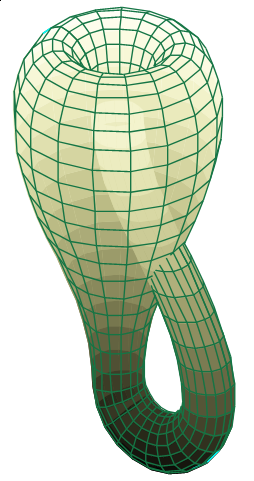
\includegraphics[scale=0.3]{klein_bottle.jpg}
  \caption{Klein Bottle}
  \label{fig:klein_bottle}
\end{figure*}

% section topological_embeddings (end)

% chapter lecture_9_jan_25th (end)

\appendix

\backmatter

\pagestyle{plain}

\nobibliography*
\bibliography{references}

\printindex

\end{document}
